\clearemptydoublepage
\chapter{Background}

\chaptermark{Background}
%What is model driven engineering
%Metamodeling: definition and tools
%Main concepts: metamodel, constraint, transformation,
%Automation in MDE
%Evolution in MDE
In this chapter, I introduce the necessary background for Model-Driven Engineering. In Section~\ref{Metamodeling}, I present the activity of metamodeling and the involved artifacts. Section~\ref{mde_automation} discusses the automation task related to the artifacts presented in Section~\ref{Metamodeling}, followed by a presentation of the evolution and co-evolution concepts in the context of Model-Driven Engineering. I finish this chapter with few main information about Large Language Models.
%define the terminology of the main concepts that we use. 
% We define the specific scope of problems addressed in this thesis
% and discuss the spectrum of problems that arise in this field. 
%TODO Terminology: Model-Driven engineering, co-evolution
% Metamodel, co-evolution, code, maintenance, refactoring

\section{Model-Driven Engineering}
\label{mde}
To develop a software, a list of specifications is given to the developers to code the final product. This approach can work in the case of small projects. When the complexity of the software increases, more efficient approaches must be adopted. Model-Driven Engineering has proven its efficiency comparing to other engineering disciplines in developing hyper-complex systems \cite{1231146}.

%\boitemagique{Model-Driven Enginereering}{
\textit{Model-Driven Engineering (MDE)} is the systematic use of models as primary artifacts during a software engineering process. The usage of models allows more abstraction that helps in managing complexity. The first appearance of MDE-like approaches started in the 80's \cite{10.1007/s10270-005-0079-0}. Till today, MDE is still adopted  and a lot of work is being done in both academia and industry \cite{Mohagheghi2009,mohagheghi2008proof,jongeling2022Structural,wortmann2020modeling}. MDE includes various Model-Driven approaches to software development, including Model-Driven Architecture, Domain-Specific Modeling and Model-Integrated Computing~\cite{10.1145/1985793.1985882}. 



%}
%TODO detaills the benefits of MDE

%Details about MDE approach 
The goal of MDE is to improve productivity, quality, and maintainability by leveraging high level abstractions throughout the development process. MDE process includes many activities: metamodeling, model verification, code generation, model transformations, implementation, testing, and documentation. The metamodeling phase implied the experts of the domain who focus on the major key aspects of the problem rather than being concerned about the underlying programming language and the implementation. Moreover, it aims to improve communication between multi-disciplinary collaborators \cite{wortmann2020modeling}.
%about major key aspects of the problem statement rather than focusing on programming.
%Metamodeling and modeling langugaes

% MEtamodel def :
The metamodel represents the main artifact in MDE, it is also a main concept in my work. There are many definitions of the concept "metamodel" that can be found in literature from Stahl et al. \cite{stahl2006model}:

\textbf{Definition 01}: \textit{A metamodel} describes concepts that can be used for modeling the model (i.e. in the instances of the metamodel).

\textbf{Definition 02}: \textit {Metamodels} are models that make statements about modeling. More precisely, a metamodel describes the possible structure of models in an abstract way, it defines the constructs of a modeling language and their relationships.
%as well as constraints and modeling rules, but not the concrete syntax of the language.

\textbf{Definition 03}: \textit{A metamodel} defines the abstract syntax and the static semantics of a modeling language. Analogously, like a written program instance (e.g., in c or java, etc.) conforms to a grammar, a model instance conforms to a metamodel.
% vice versa, each formal language, such as Java or UML, possesses a metamodel.

Seidewitz \cite{seidewitz2003models} gives another commonly used definition of \textit{metamodels} in MDE:

\textbf{Definition 04}: \textit{A metamodel} is a specification model for a class of systems under study where each system under study in the class is itself a valid model expressed in a certain modeling language.

\section{Metamodeling}
\label{Metamodeling}
%definition, related tasks and artifacts, usages in different languages, tools
%%
\textit{Metamodeling} is the process of metamodel creation. Metamodeling is done thanks to metamodeling languages (that is in turn described by a meta-metamodel) as illustrated in Figure~\ref{fig:mofmodellevels}.

Metamodeling must gather the whole  knowledge that is required to define, precise, and deal with MDE challenges in its different tasks \cite{wortmann2020modeling}, related to other artifacts shown in Figure~\ref{fig:mde_ecosystem}. The main metamodeling-related tasks are:

%DSL/ sftware language 
%Construction of domain-specific modeling languages (DSLs): 
%The metamodeling activity includes other tasks:
\begin{figure}[htbp]
	\begin{center}
		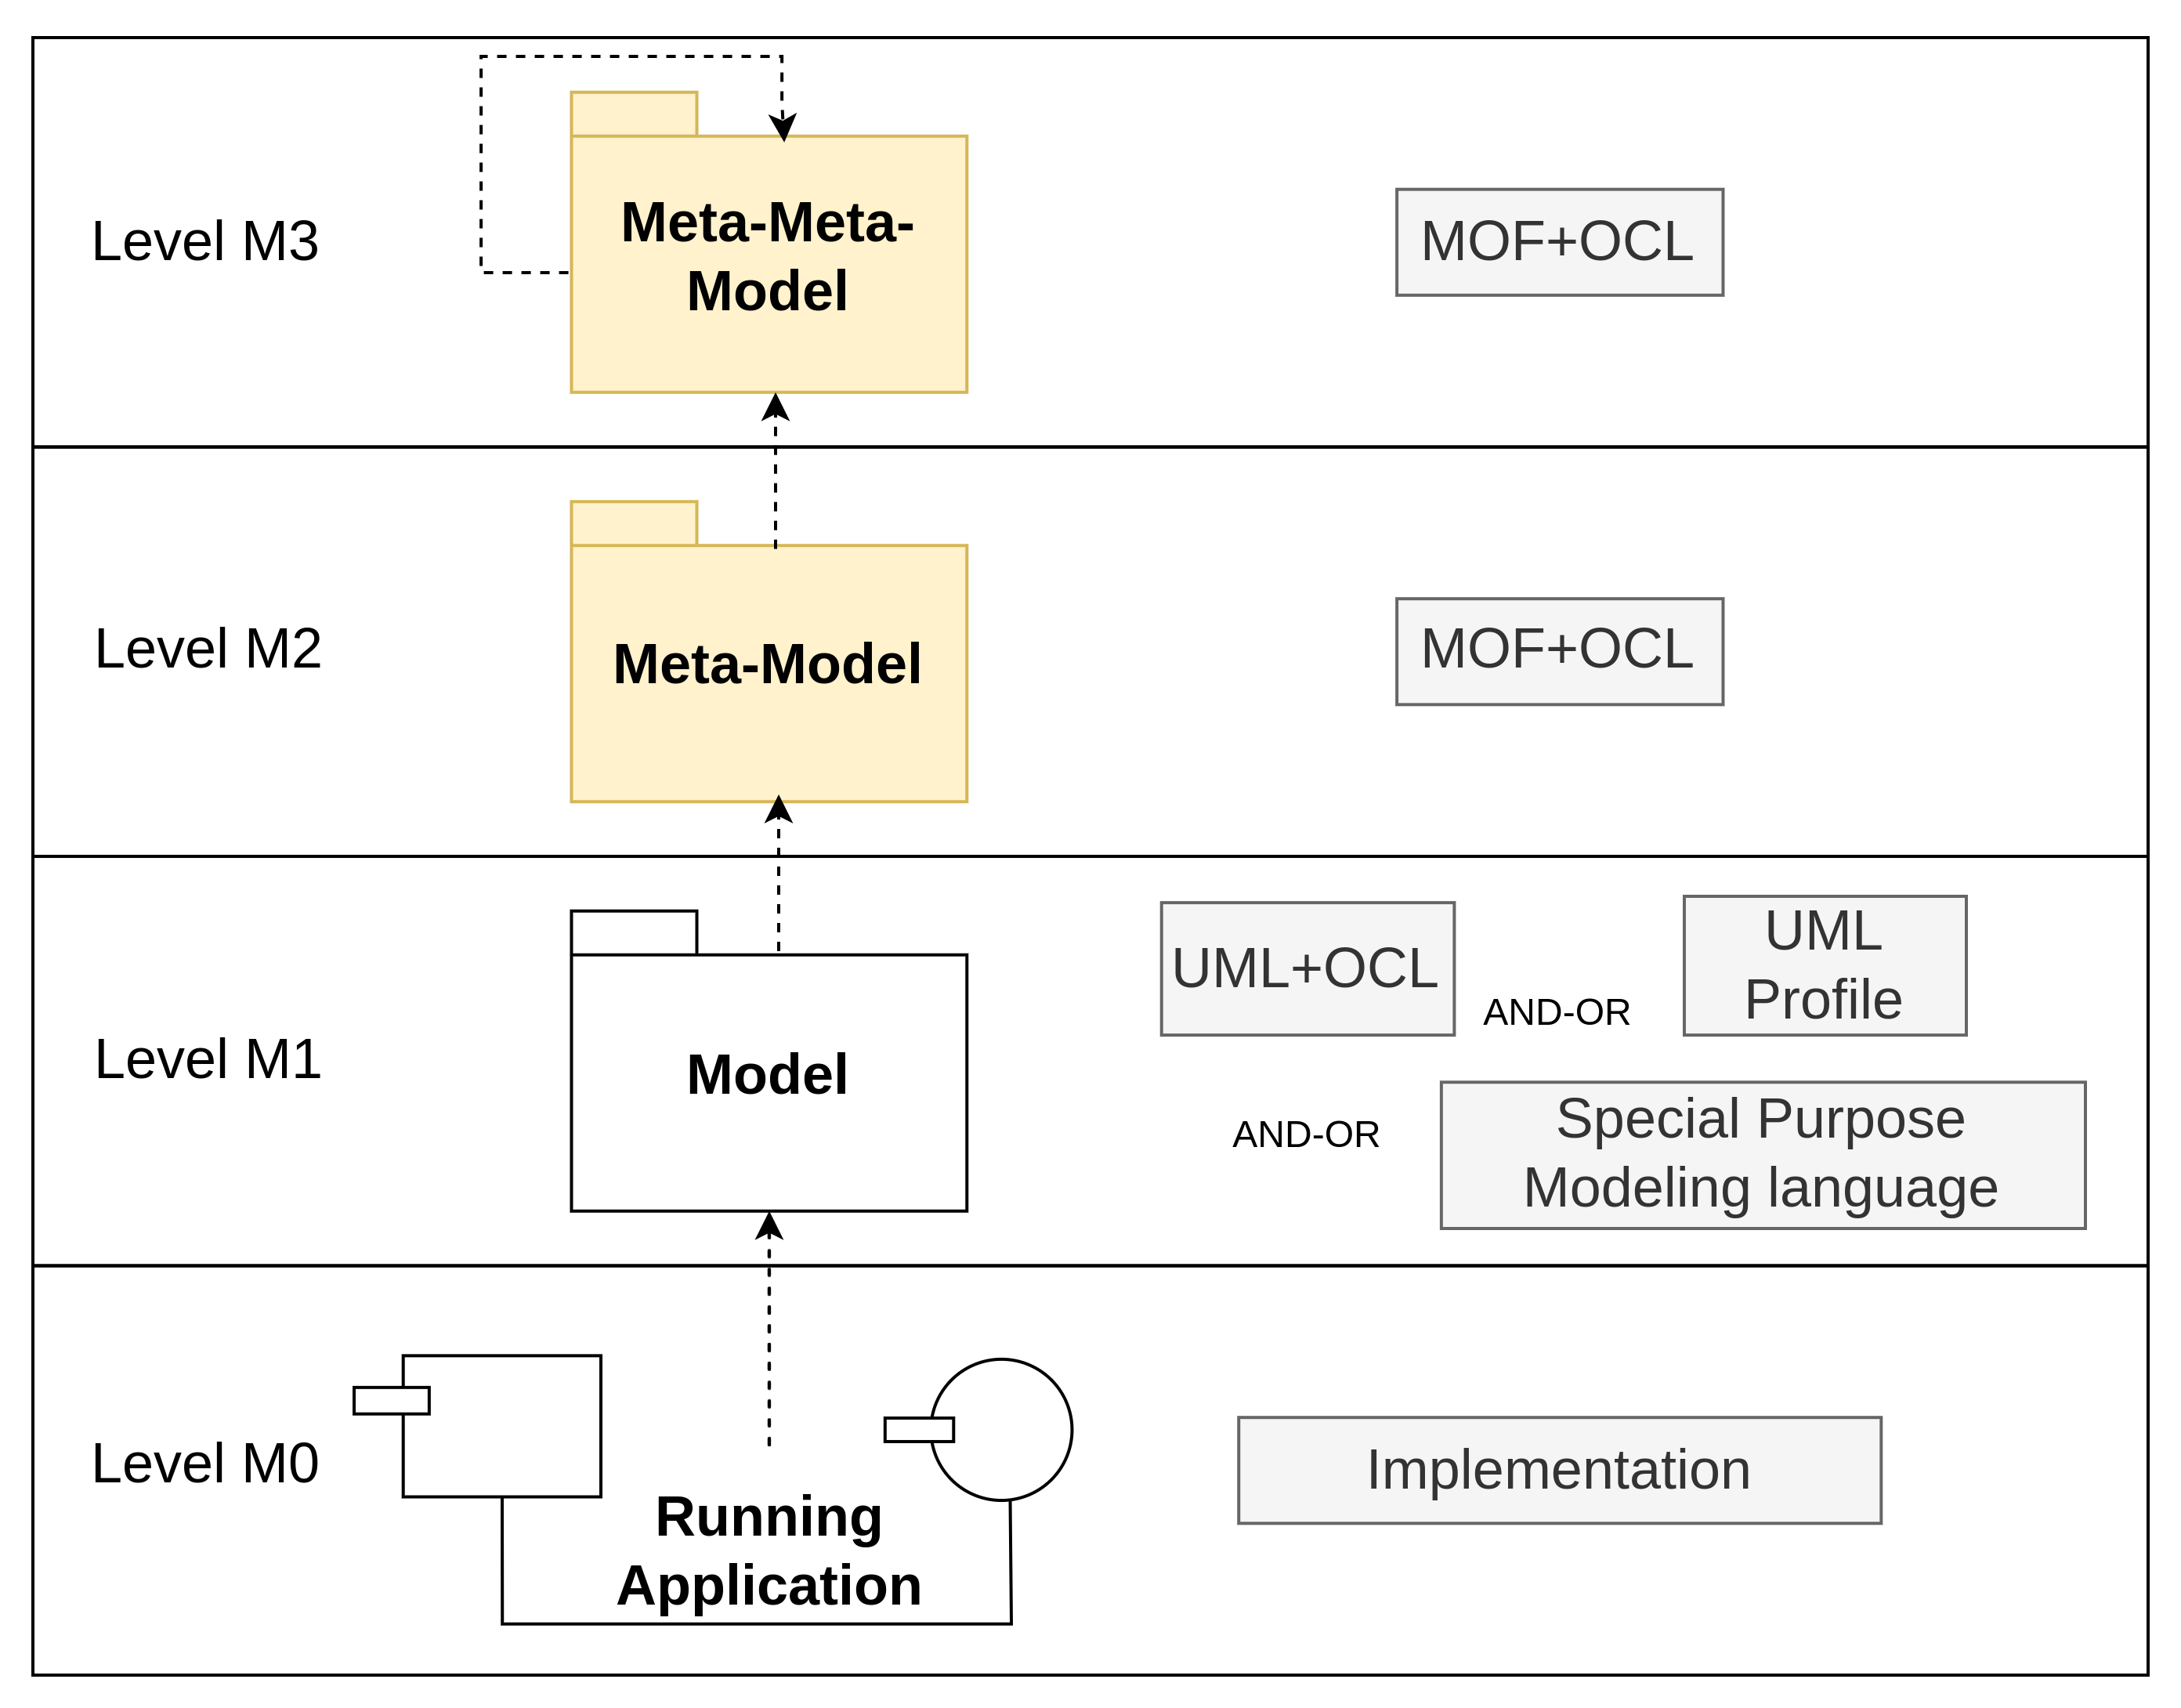
\includegraphics[width=0.6\linewidth]{./pics/soaPics/mofmodellevels2.png}
	\end{center}
	\caption{MDA’s Modeling Level Hierarchy}
	%	{\footnotesize Titre plus long avec des explications.}
	\label{fig:mofmodellevels}
\end{figure}
\begin{figure}[htbp]
	\begin{center}
		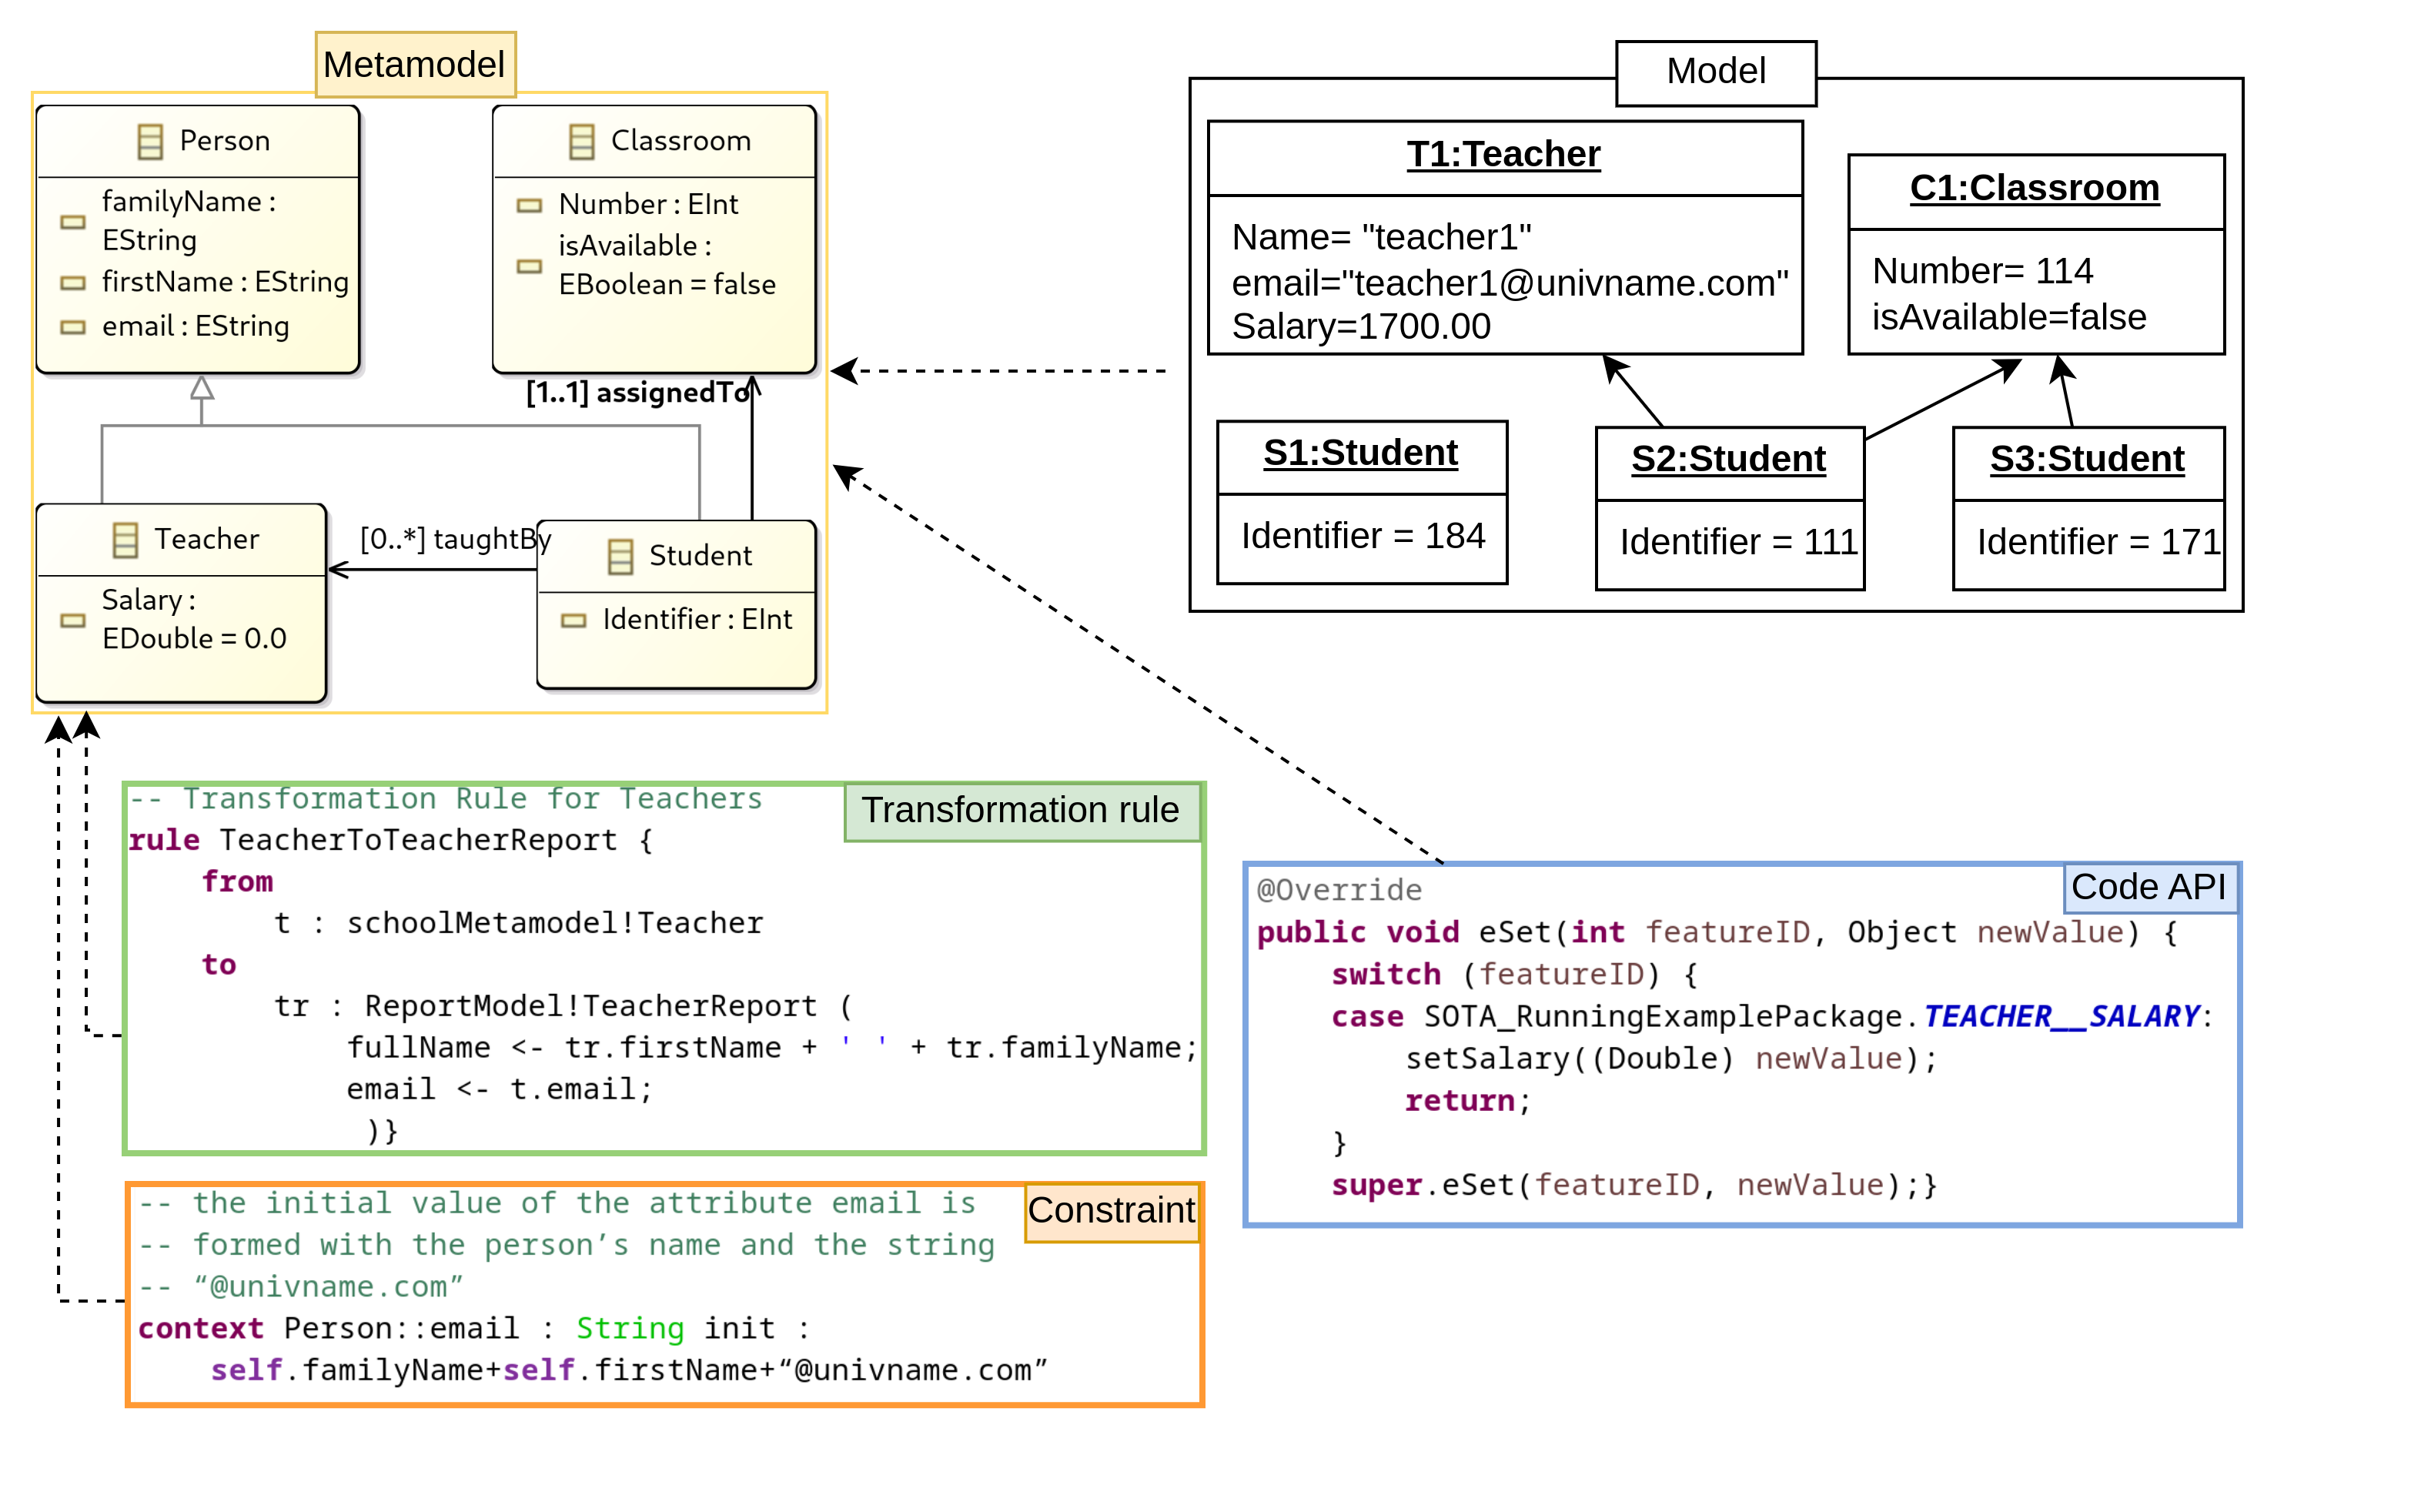
\includegraphics[width=\linewidth]{./pics/soaPics/notabstractecosystem2.png}
	\end{center}
	\caption{MDE Ecosystem}
	%	{\footnotesize Titre plus long avec des explications.}
	\label{fig:mde_ecosystem}
\end{figure}
\begin{itemize}
\item The construction of metamodel itself: it describes the abstract syntax of target software languages or  solution system.
\item Model validation: models are validated against the constraints defined in the metamodel. 
\item Model-to-model transformations: such transformations are defined as mapping rules between source model and a target model .
\item Code generation: it consists of automatically producing source code from models, bridging the gap between high-level abstractions and executable software.
\item Tool integration: based on the metamodel, modeling tools can be adapted to the respective domain. 
\end{itemize}


In the context of Domain-Specific Languages,  represent an essential application of metamodels in practice. A DSL is a specialized language tailored to the needs and constructs of a specific domain, enabling domain experts to express solutions at a higher level of abstraction without delving into general-purpose programming complexities. These languages are typically defined by a metamodel that establishes their syntax and semantics, ensuring consistency and precision. By leveraging metamodeling to create DSLs, engineers can align software artifacts closely with domain-specific requirements, enhancing clarity, maintainability, and automation potential in the software development process \cite{volter2013model}. 

%The metamodel is the basis for the automated, tool-supported processing of models. On the other hand, a suitable concrete syntax is the interface to the modeler and its quality decides what degree of readability the models have \cite{stahl2006model}.

%Metamodeling tools/languages/techniques examples :

%// Add figure?

Metamodeling languages are classified into two categories, namely linguistic and ontological \cite{gavsevic2007metamodeling}. Linguistic metamodeling represents a way for defining modeling languages and their primitives (e.g., Object, Class, MetaClass) on the layer of a metamodel. Ontological metamodeling aims to represent domain knowledge accurately. It is concerned with semantics and meaning, e.g., OWL\footnote{https://www.w3.org/TR/owl-features/}. Linguistic metamodeling aims to define a language for creating models. it is concerned with syntax and structure.
I can use a different classification by purpose: General Purpose Modeling Languages and Domain-Specific Modeling Languages~\cite{de2012domain}. General Purpose Modeling Languages as for example : UML and its variants, generic metamodeling frameworks, such as MOF \footnote{https://www.omg.org/mof/}, and Ecore \footnote{https://eclipse.dev/modeling/emft/search/concepts/subtopic.html}. As examples of DSLs, I cite sysML and EXPRESS DSL~\cite{wortmann2020modeling}.

In MDE, there are language workbenches that are used for language creation, such as Xtext, MetaEdit+ \cite{wortmann2020modeling}.
% Add figure for above languages/techniques/frameworks

%\textbf{Generated artifacts, artifacts linked to the metamodel}


%Metamodel is the backbone in model driven engineering. 
In the language modeling ecosystem, other artifacts are created by the mean of the metamodel. By definition, a model is an instance of a metamodel, which means that the metamodel defines the concepts with which a model can be created. The created models can also be validated through a set of constraints to check the models' correctness. Constraints are written in Object Constraint Language. They precise specifications on the model that cannot be  expressed by diagrammatic notation. In order to save effort and avoid errors, models transformation is one of the common automated tasks in Model-driven engineering. Model transformation are expressed in  Transformation Languages for example, ATL). A transformation consists of a set of rules that map the source metamodel elements to the metamodel target’s elements. All of these artifacts have their specific tools and represent an important topic of research in MDE.

%// Add example of Metamodel+ model+constraint+transformation ?

%ex constraint : the age of a person is not negative, a person is younger than its parents
%Automation in the ecosystem
%code gen 
%tests
\section{Automation in the MDE ecosystem}
\label{mde_automation}
%Brief description about automated tasks in MDE.
 Automation plays a pivotal role within the MDE ecosystem. It is considered as one of the most important advantages of MDE. This section explores the significance of automation in MDE, particularly in the code generation activity and during the evolution of the metamodel cornerstone artifact.
 
 % This section explores also the impact of automation on the development lifecycle.% and key strategies for achieving efficient model-driven processes.

\subsection{Code Generation}

One of the most important activities in MDE is the code generation activity. It is recurrent, and its automation enhances the productivity and the cost. For example, Eclipse Modeling Framework built-in code generator allows to generated a java API from an Ecore metamodel. The generated code API structure and technical choices are done to fit Java programming language and Model-Driven Engineering abstraction standards and principles (e.g., each metaclass is used to generate an interface and concrete implementation class that extends the generated interface, pattern observer).
% to have an efficient as possible
 The annotation \textit{@generated} is used to mark generated interfaces, classes, methods, and fields. This annotation can be used to differentiate the generated code from the manually written one.

In Eclipse Modeling Framework, two model resources (files) are manipulated: the .ecore file that contains  XMI serialization of the Ecore model and the .genmodel for the serialized generator model. The Ecore file is the document that contains the metamodeled main concepts that are used in code generation process.

%\textcolor{blue}{Develop this paragraph?}
\subsection{Software evolution}
From operating systems to mobile apps, software is the cornerstone of modern innovation. However, software does not remain static, it evolves over time to meet new demands, address challenges, and incorporate advancements. Here some numbers showing how much a software can evolve. Let's take Eclipse Modeling Framework (EMF) as a first example from MDE context. EMF\footnote{\url{https://github.com/eclipse-emf/org.eclipse.emf}} has~65 releases, with~10374 commits, and more than~823k lines of code. Another example from MDE is UML \footnote{\url{https://github.com/eclipse-uml2/uml2}} with~2806 commits and more than~716k lines of code. The third example is Linux kernel \footnote{\url{https://github.com/torvalds/linux}} with~1324878 commits and~40 million lines of code. Then
chromium \footnote{\url{https://github.com/chromium/chromium.git}} with~1524157 commits and more than~32 million lines of code. The last example is
cpython \footnote{\url{https://github.com/python/cpython}} with~124936 commits, more than~350k lines of C code and~600k lines of python code.
\begin{figure}[t]
	\begin{center}
		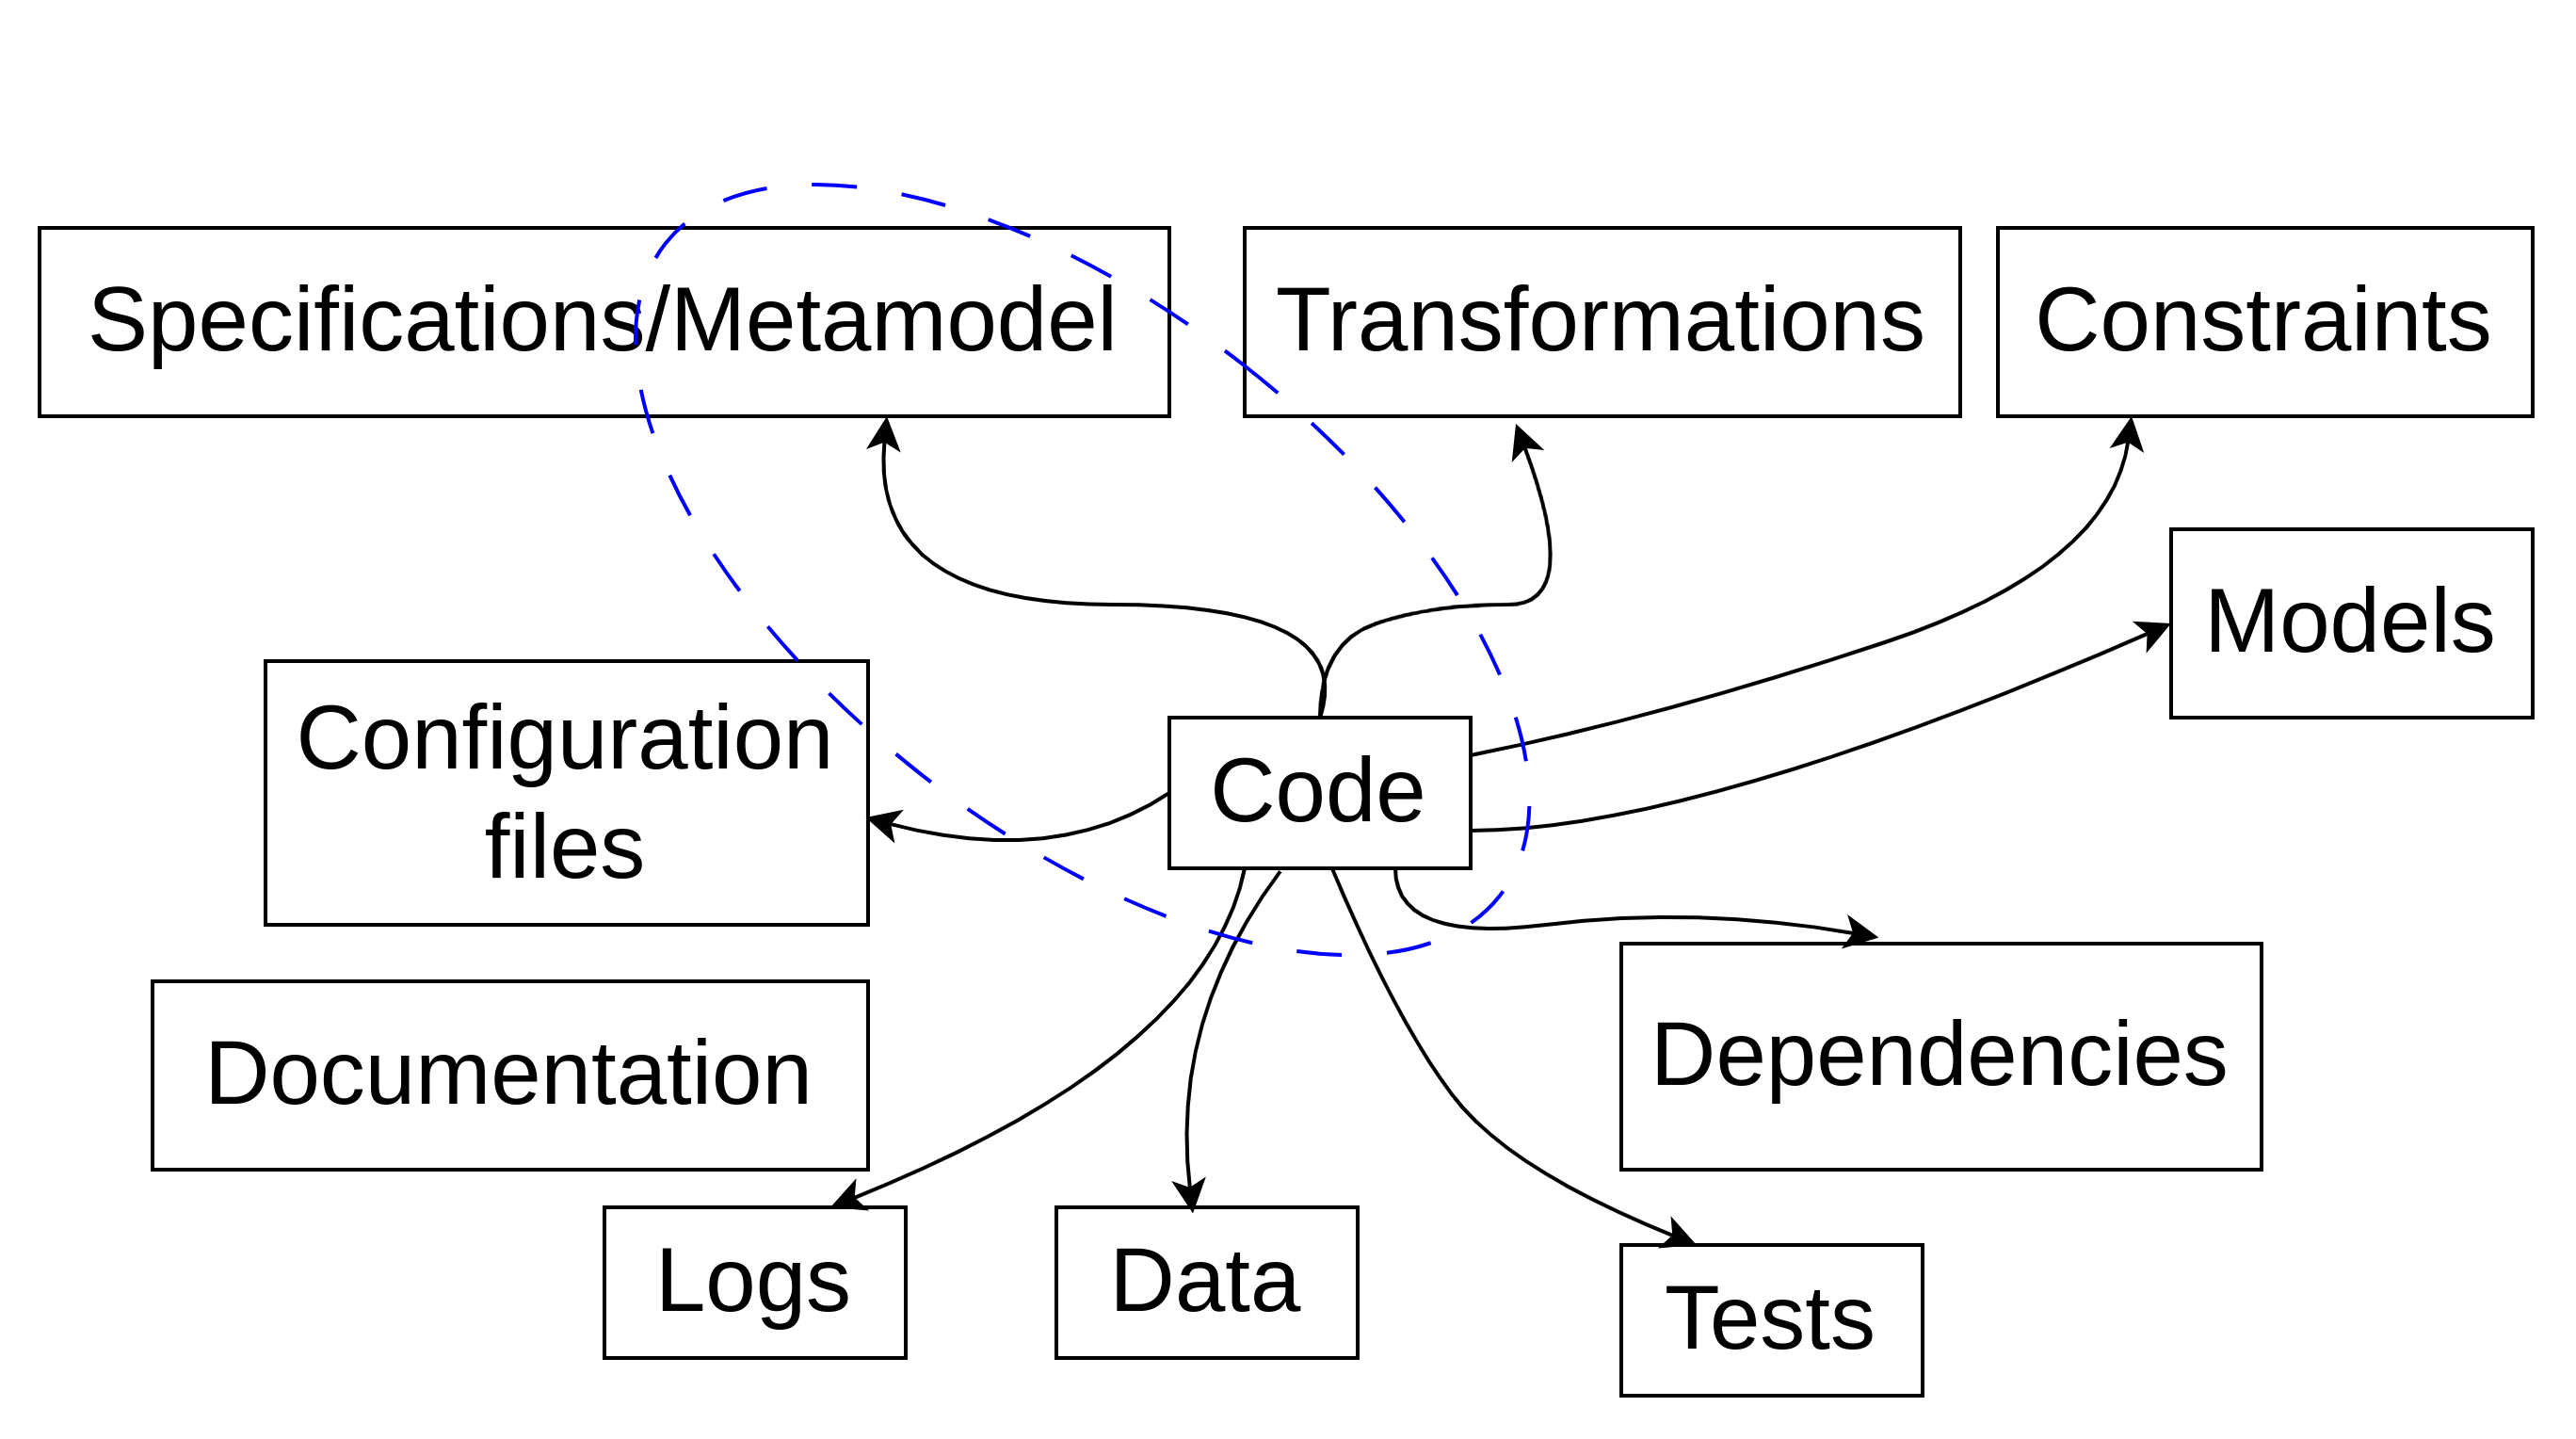
\includegraphics[width=0.6\linewidth]{./pics/soaPics/softwareartifacts.png}
	\end{center}
	\caption{software artifacts}
	\label{fig:softwareartifacts}
\end{figure}
During the software development process, software artifacts are meant to be changed, due to many reasons: client requirements and domain specifications, software maintenance, or bug correction. The evolution can impact one artifact ore more in the software ecosystem (Figure \ref{fig:softwareartifacts}). Like any other software system, modeling languages are the subject of an inevitable evolution, during their process of building, multiple versions are developed, tested, and adapted until a stable version is reached. 

Different types of evolution are categorized depending on the impact and purpose of the applied modifications \cite{lientz1980software,Swanson1976}:
\begin{itemize}
	
	\item  Corrective: aims to correct discovered problems and inconsistencies, such as processing failures, performance failures, or implementation failures by applying a set of reactive modifications of a software product.  
	
	\item  Adaptive: in case of changing environment, such as changes in data environment or processing environment, this evolution aims to keep a software product usable.
	
	\item Perfective: this evolution aims to improve functionalities, to enhance the performance, reliability, or to increase the maintainability of a software.  
	
\end{itemize}
%It is unavoidable to change, whether to answer to requirement modifications and/or technological progress.
The term \textit{Evolution} can be refined as the literature presents various related terms like: Maintenance, Refactoring, and \textbf{Co-evolution}, which are different types of modifications that could be applied on a software. There is no clear definition for each of them, however, in figure \ref{fig:evolutiontypes} I describe the relationship between these terms by intent and by artifacts on which the task is applied.

%/Why we need to perform evolution ?
%examples?
%TODO Add defs references

\textbf{Evolution}: any adaptation that occurs in the software in response to new requirements. These requirements are the consequence of the past experience of the users that feeds the developers' learning. \cite{bennett2000software}. 

\textbf{Maintenance}: It is modifying a software product after delivery to correct faults, to improve performance, or to adapt the product to a changing environment \cite{schneidewind1987state}.

\textbf{Refactoring}: It is an oriented object term, that means behavior-preserving modifications of software, to make it easier to understand and to change or to make it less susceptible to errors when future changes are introduced \cite{mens2004survey}. 

\textbf{Co-evolution}: It consists of the process of adapting and correcting a set of artifacts $A_1$, $A_2$, ...$A_N$ in response to the evolution of an artifact B on which $A_1$, $A_2$, ...$A_N$  strongly depend, for example the co-evolution of models with the evolving metamodel as used in Kessentini et al. paper \cite{Kessentini2016automated}, and the co-evolution of API/client as used in Eilertsen et al. paper \cite{8443581}. The term "Coupled evolution" was also mentionned in the work of Herrmannsdoerfer et al. in the context of metamodel and model co-evolution \cite{herrmannsdoerfer2009cope}

%\begin{figure}[htbp]
%	\begin{center}
%		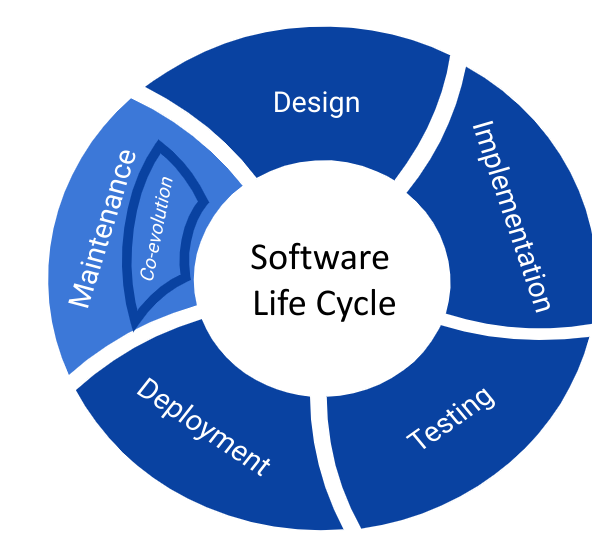
\includegraphics[width=0.6\linewidth]{./pics/soaPics/solicy.png}
%	\end{center}
%	\caption{Software Life Cycle ( not sure to include)}
%	{\footnotesize Titre plus long avec des explications.}
%	\label{fig:softwarelifecyle}
%\end{figure}



\begin{figure}[t]
	\begin{center}
		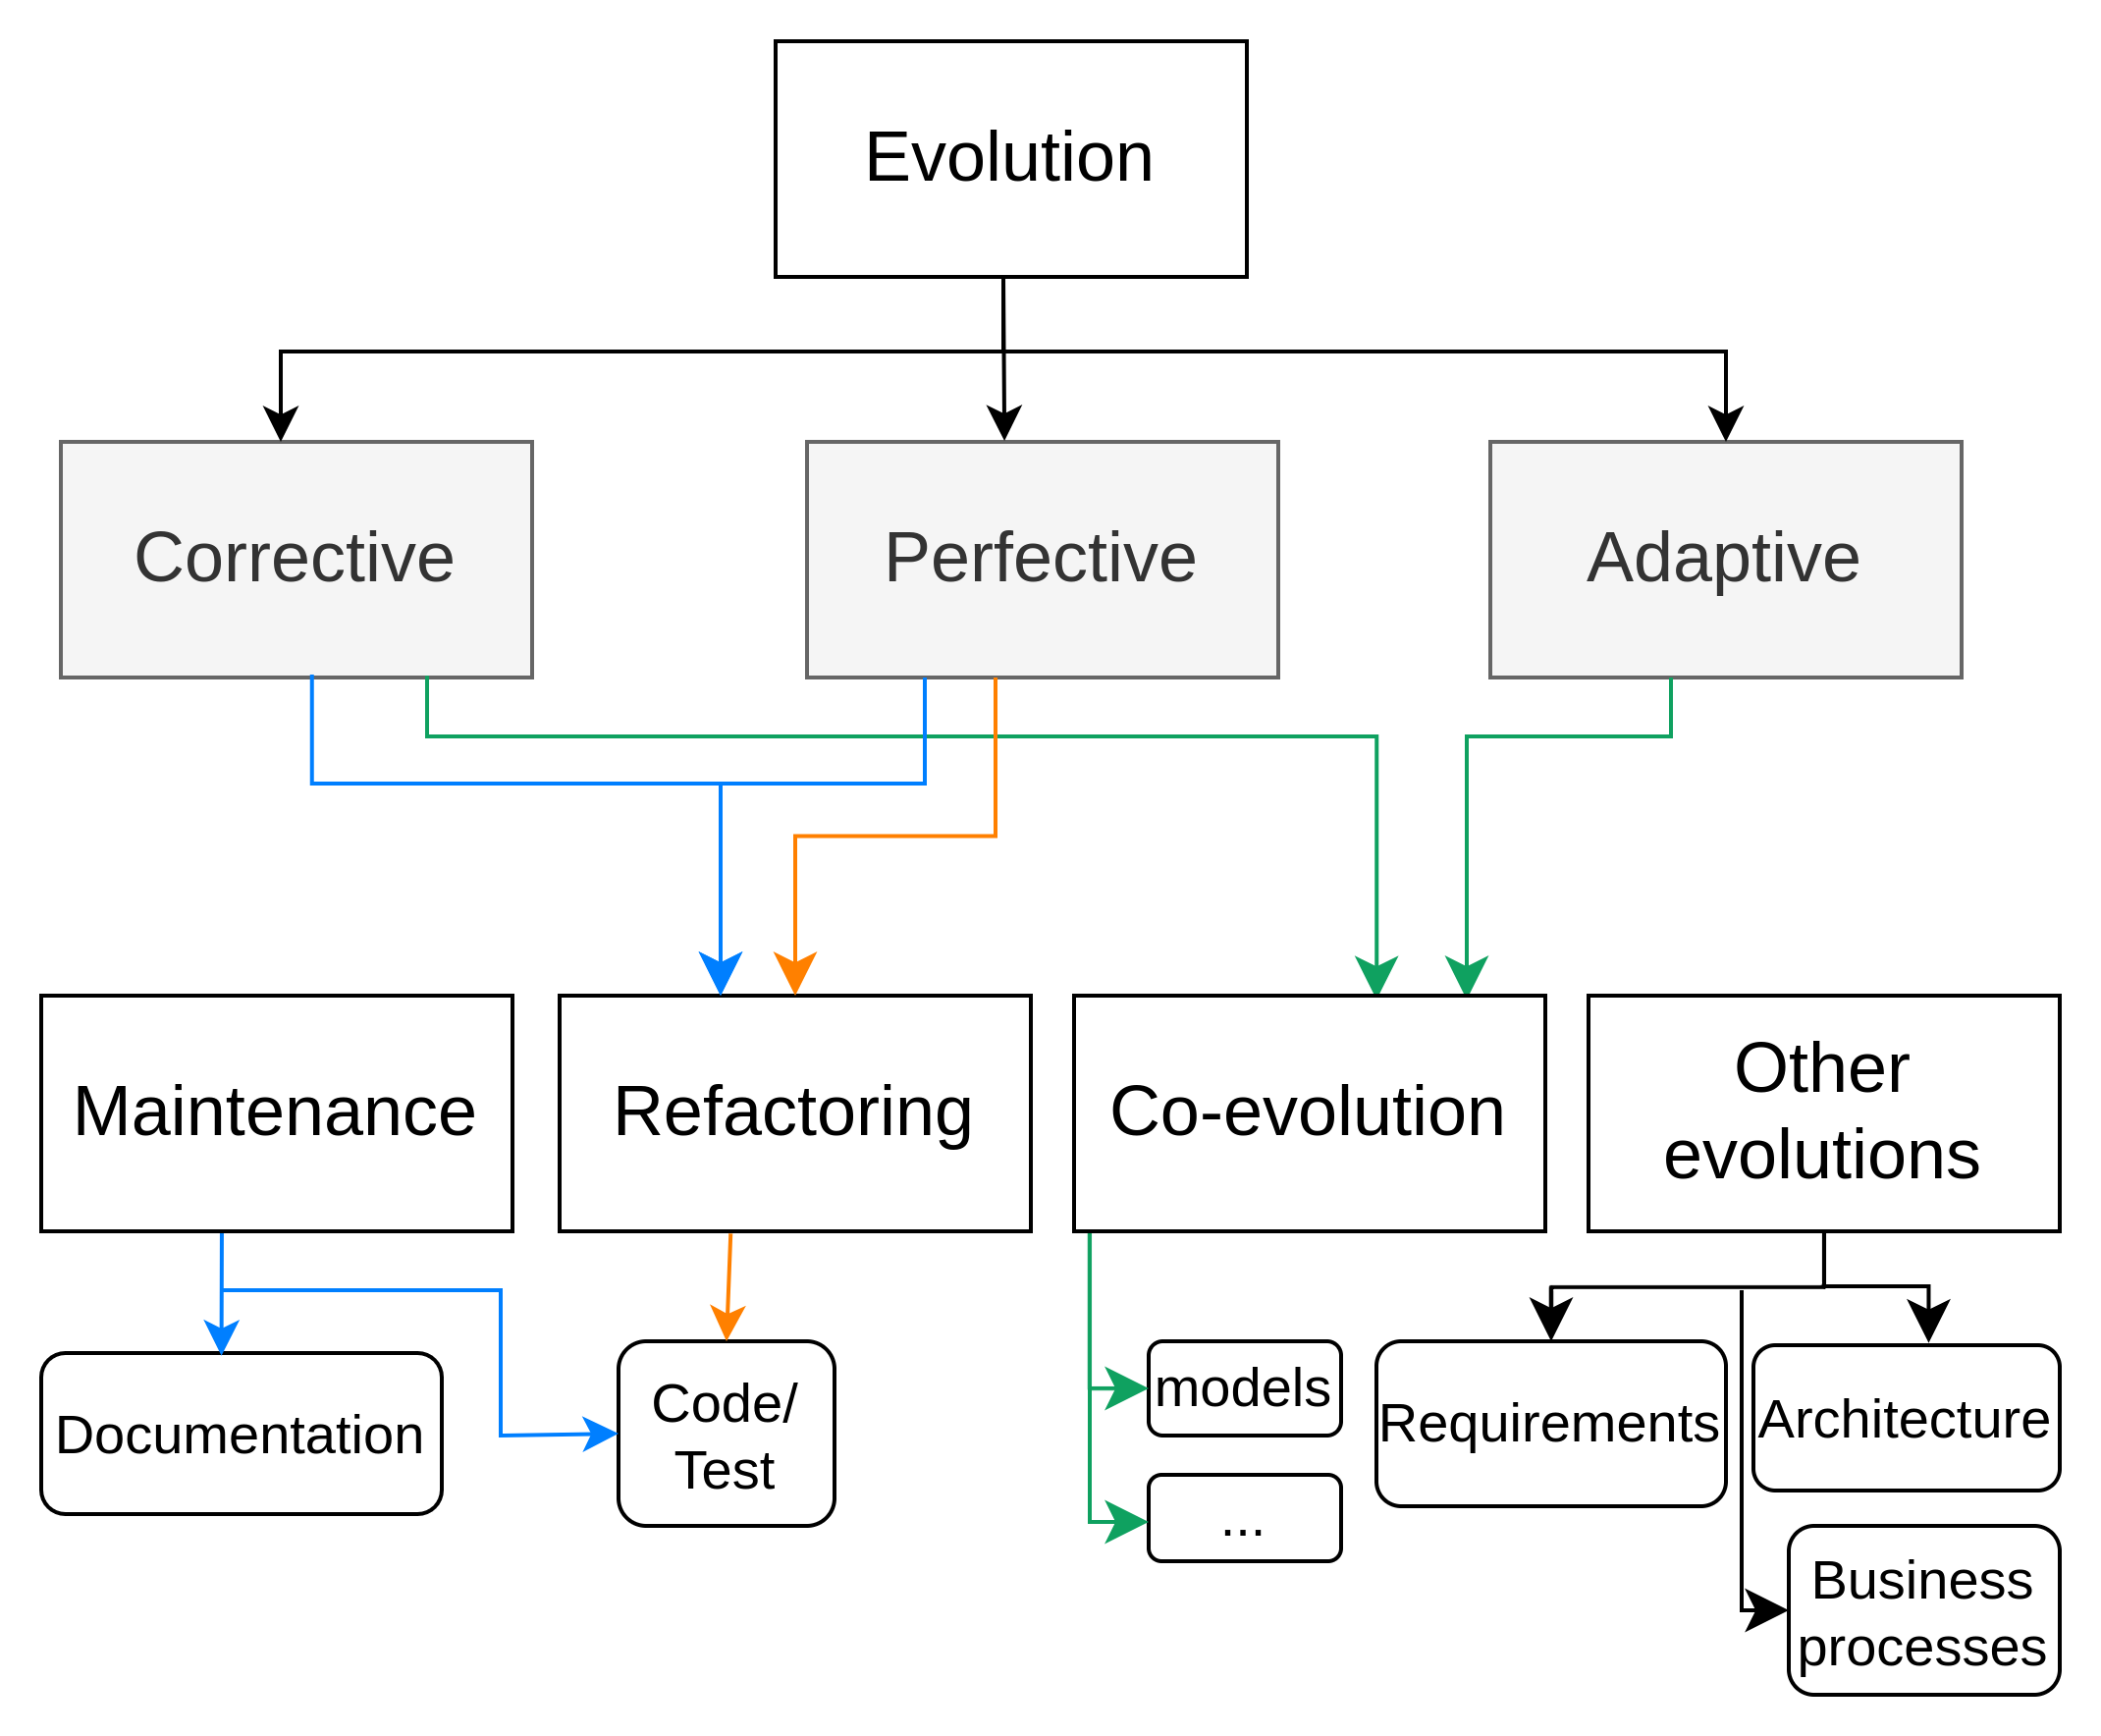
\includegraphics[width=0.6\linewidth]{./pics/soaPics/evolutiontypes.png}
	\end{center}
	\caption{Evolution related terminology}
	%	{\footnotesize Titre plus long avec des explications.}
	\label{fig:evolutiontypes}
\end{figure}

\section{Large Language Models}
In this section, I outline the fundamental concepts related to Large Language Models, namely Transformer models and prompt engineering. I give a short historical view to understand the added value of using LLMs in my third contribution (cf. Chapter ?).

\subsection{From Transformer Models to Large Language Models}

%Rule-based and hand-crafted solutions are rigid and hard to scale.
Machine learning field introduced statistical models that learn from input data. As an improvement of traditional machine learning approaches, neural networks brought breakthroughs in image and speech recognition, inspiring their application to Natural Language Processing (NLP). A markup point in the history of machine learning is The Attention Mechanism \cite{10.5555/3295222.3295349}. It allows models to focus on relevant parts of input sequences, significantly enhancing translation and comprehension tasks.
This mechanism allows the model to weigh the importance of all words in a sequence simultaneously, leading to: 1) Parallel processing for a faster computation, and 2) Better handling of long-range dependencies. After neural networks and Attention mechanism application in NLP, the transformer models appearance first in 2018, marked by the emergence of BERT and its variations \cite{DBLP:journals/corr/abs-2302-09419}.


%Bert def and caract vs traditional models)
\textbf{BERT} (Bidirectional Encoder Representations from Transformers) is an encoder-only transformer model owned by Google \cite{devlin2019bertpretrainingdeepbidirectional}. Regarding data corpus, BERT is pre-trained from  Wikipedia and Google’s BooksCorpus. Another remarkable model is \textbf{BART} (Bidirectional and Auto-Regressive Transformers). It was introduced by Lewis et al. \cite{lewis2019bartdenoisingsequencetosequencepretraining}.
Unlike BERT’s encoder-only design, BART’s architecture is a sequence-to-sequence model, featuring both encoder and decoder components.
In 2018, OpenAPI has launched another large scale pre-trained transformer model: GPT, then \textbf{GPT-3} in 2020 \cite{10113601}.


 

%BERT, BART, and GPT 
%main doc :Utilizing Large Language Models for Question Answering in Task-Oriented Dialogues)

Note that in the field of LLM, new approaches are being developed at a rapid pace. Thus, rather then latest models, I selected models that have marked a turning point in the history of LLMs: BERT, BART, and GPT to include in this short LLM background. No global and detailed comparison between GPT, BERT, and BART is established. However, some works have conducted targeted comparisons in specific context. For example, Yokoyama et al. compare between Chatgpt and BERT in security bug identification topic \cite{10685583}. Table \ref{table:bertvsbartvsgpt3} summarizes the key differences between BERT, BART, and GPT-3 depending on: their architecture, learning data, number of parameters, performance speed, application domain in which the model is most efficient, and the respective organizations that created them~\cite{DBLP:journals/corr/abs-2302-09419,lewis2019bartdenoisingsequencetosequencepretraining}.
%https://scholar.google.fr/scholar?as_q=comparison+BERT+chatgpt&as_epq=&as_oq=&as_eq=&as_occt=title&as_sauthors=&as_publication=&as_ylo=&as_yhi=&hl=fr&as_sdt=0%2C5



%Add the comparative table with BART column : https://updf.com/fr/chatgpt/bert-vs-gpt/
\begin{table}[h]
	\vspace{-1.2cm}
	\caption{Comparison BERT, BART, and GPT-3} 
	\label{table:bertvsbartvsgpt3}
\hspace{-2cm}
\begin{tabular}{ | m{2.5cm}| m{4cm}| m{4.5cm} |m{5.5cm} |  } 

	\hline
	\textbf{Functionality}& \textbf{BERT} & \textbf{BART} &\textbf{GPT-3} \\ 
	\hline\hline
	\textbf{Architecture} & Bidirectional encoder-only model that considers both left and right contexts when making predictions. &  Encoder-decoder model, Bidirectional encoder with left-to-right autoregressive decoder it considers both left and right contexts when making predictions. &The autoregressive model generates text by predicting the next word in a sequence based on the preceding words \\ 
	\hline
		\textbf{Data} & Learning on data from sources such as English Wikipedia and BookCorpus 11038 books). & Learning from a combination of books and Wikipedia data &  extremely large corpus of English text data extracted from millions of web pages and then fine-tuned using Reinforcement Learning from Human Feedback (RLHF) \\ 
	\hline
		\textbf{Number of parameters }& $BERT_{base}$ 110 m parameters  $BERT_{large}$ 340 million parameters, a relatively smaller number than GPT-3. & $BART_{base}$ contains 139 million parameters and $BART_{large}$ contains around 400 million parameters&175 billion parameters, far more than any other language model.\\
		\hline
			\textbf{Performance speed?}& faster than BART and GPT-3
			.& Decoding step and the number of parameters make it slower than BERT& the slowest one, because of the number of parameters, size of data, and the complex architecture.\\
		\hline
			\textbf{Application (domain)}&Top performance on a range of tasks, including text classification.
			Requires further fine-tuning and learning to adapt to new domains and tasks.&particularly effective when fine-tuned for downstream NLP tasks, especially text generation&It has shown remarkable performance on a wide range of natural language processing tasks.
			Can be generalized to new domains thanks to learning in a few steps, and adapted to new tasks thanks to transfer learning.\\
			\hline

\textbf{Origin organisation}&Google AI&Facebook AI& OpenAI\\
\hline		
\end{tabular}
	\end{table}
%Large scale pre-training, high scalability.


\subsection{Prompt Engineering}


\textbf{Definition -- Prompt Engineering.} It consists of techniques that are used to converse with LLMs. As a subdomain of LLMs field, it represents an active and rapidly evolving area of study. Frieder et al. confirm the impact of having a correct prompt structure in the capability of LLMs' problems resolution \cite{10.5555/3666122.3667327}. 
Although GPT-3 may have popularized these prompt engineering techniques \cite{10.5555/3495724.3495883}, other LLMs are capable of these generalization techniques, such as PaLM \cite{10.5555/3648699.3648939} and Chinchilla \cite{10.5555/3600270.3602446}.

Here I define two popular categories of prompt-engineering techniques: zero-shot/few-shot prompting and Chain-of-Thought reasoning:
\begin{itemize}
	\item Few-shot/zero-shot prompting: In few-shot prompting, the prompt is enriched with one or more examples of the task in the prefix before being asked to perform the task on new data. These examples serve as a way to prime the model to produce the desired output. In zero-shot prompting, no example is provided \cite{brown2020languagemodelsfewshotlearners,10.1145/3560815}.
	
%	Whatpu example nop , to demo next
	
	\item Chain-of-Thought reasoning: enables complex reasoning capabilities through intermediate reasoning steps. it can be combined with few-shot prompting to get better results on more complex tasks that require reasoning before responding \cite{10.5555/3600270.3602070}.
	
	Note that other techniques can be found in Liu et al. systematic survey of prompting methods in \cite{10.1145/3560815}, and in this prompting guide website \footnote{\url{https://www.promptingguide.ai/techniques}}.
	
	Let's take an example for the prompt "If Alice has 5 apples and gives 3 to Bob, how many apples does Alice have left?". Figure \ref{fig:fewshotexample} shows the prompt content in the case of few-shot prompting, and Figure \ref{fig:cotexample} shows the chain-of thought reasoning for the same prompt.
	
	
	\begin{figure*}[t!]
		\centering
		\begin{subfigure}[t]{0.5\linewidth}
			%\centering
			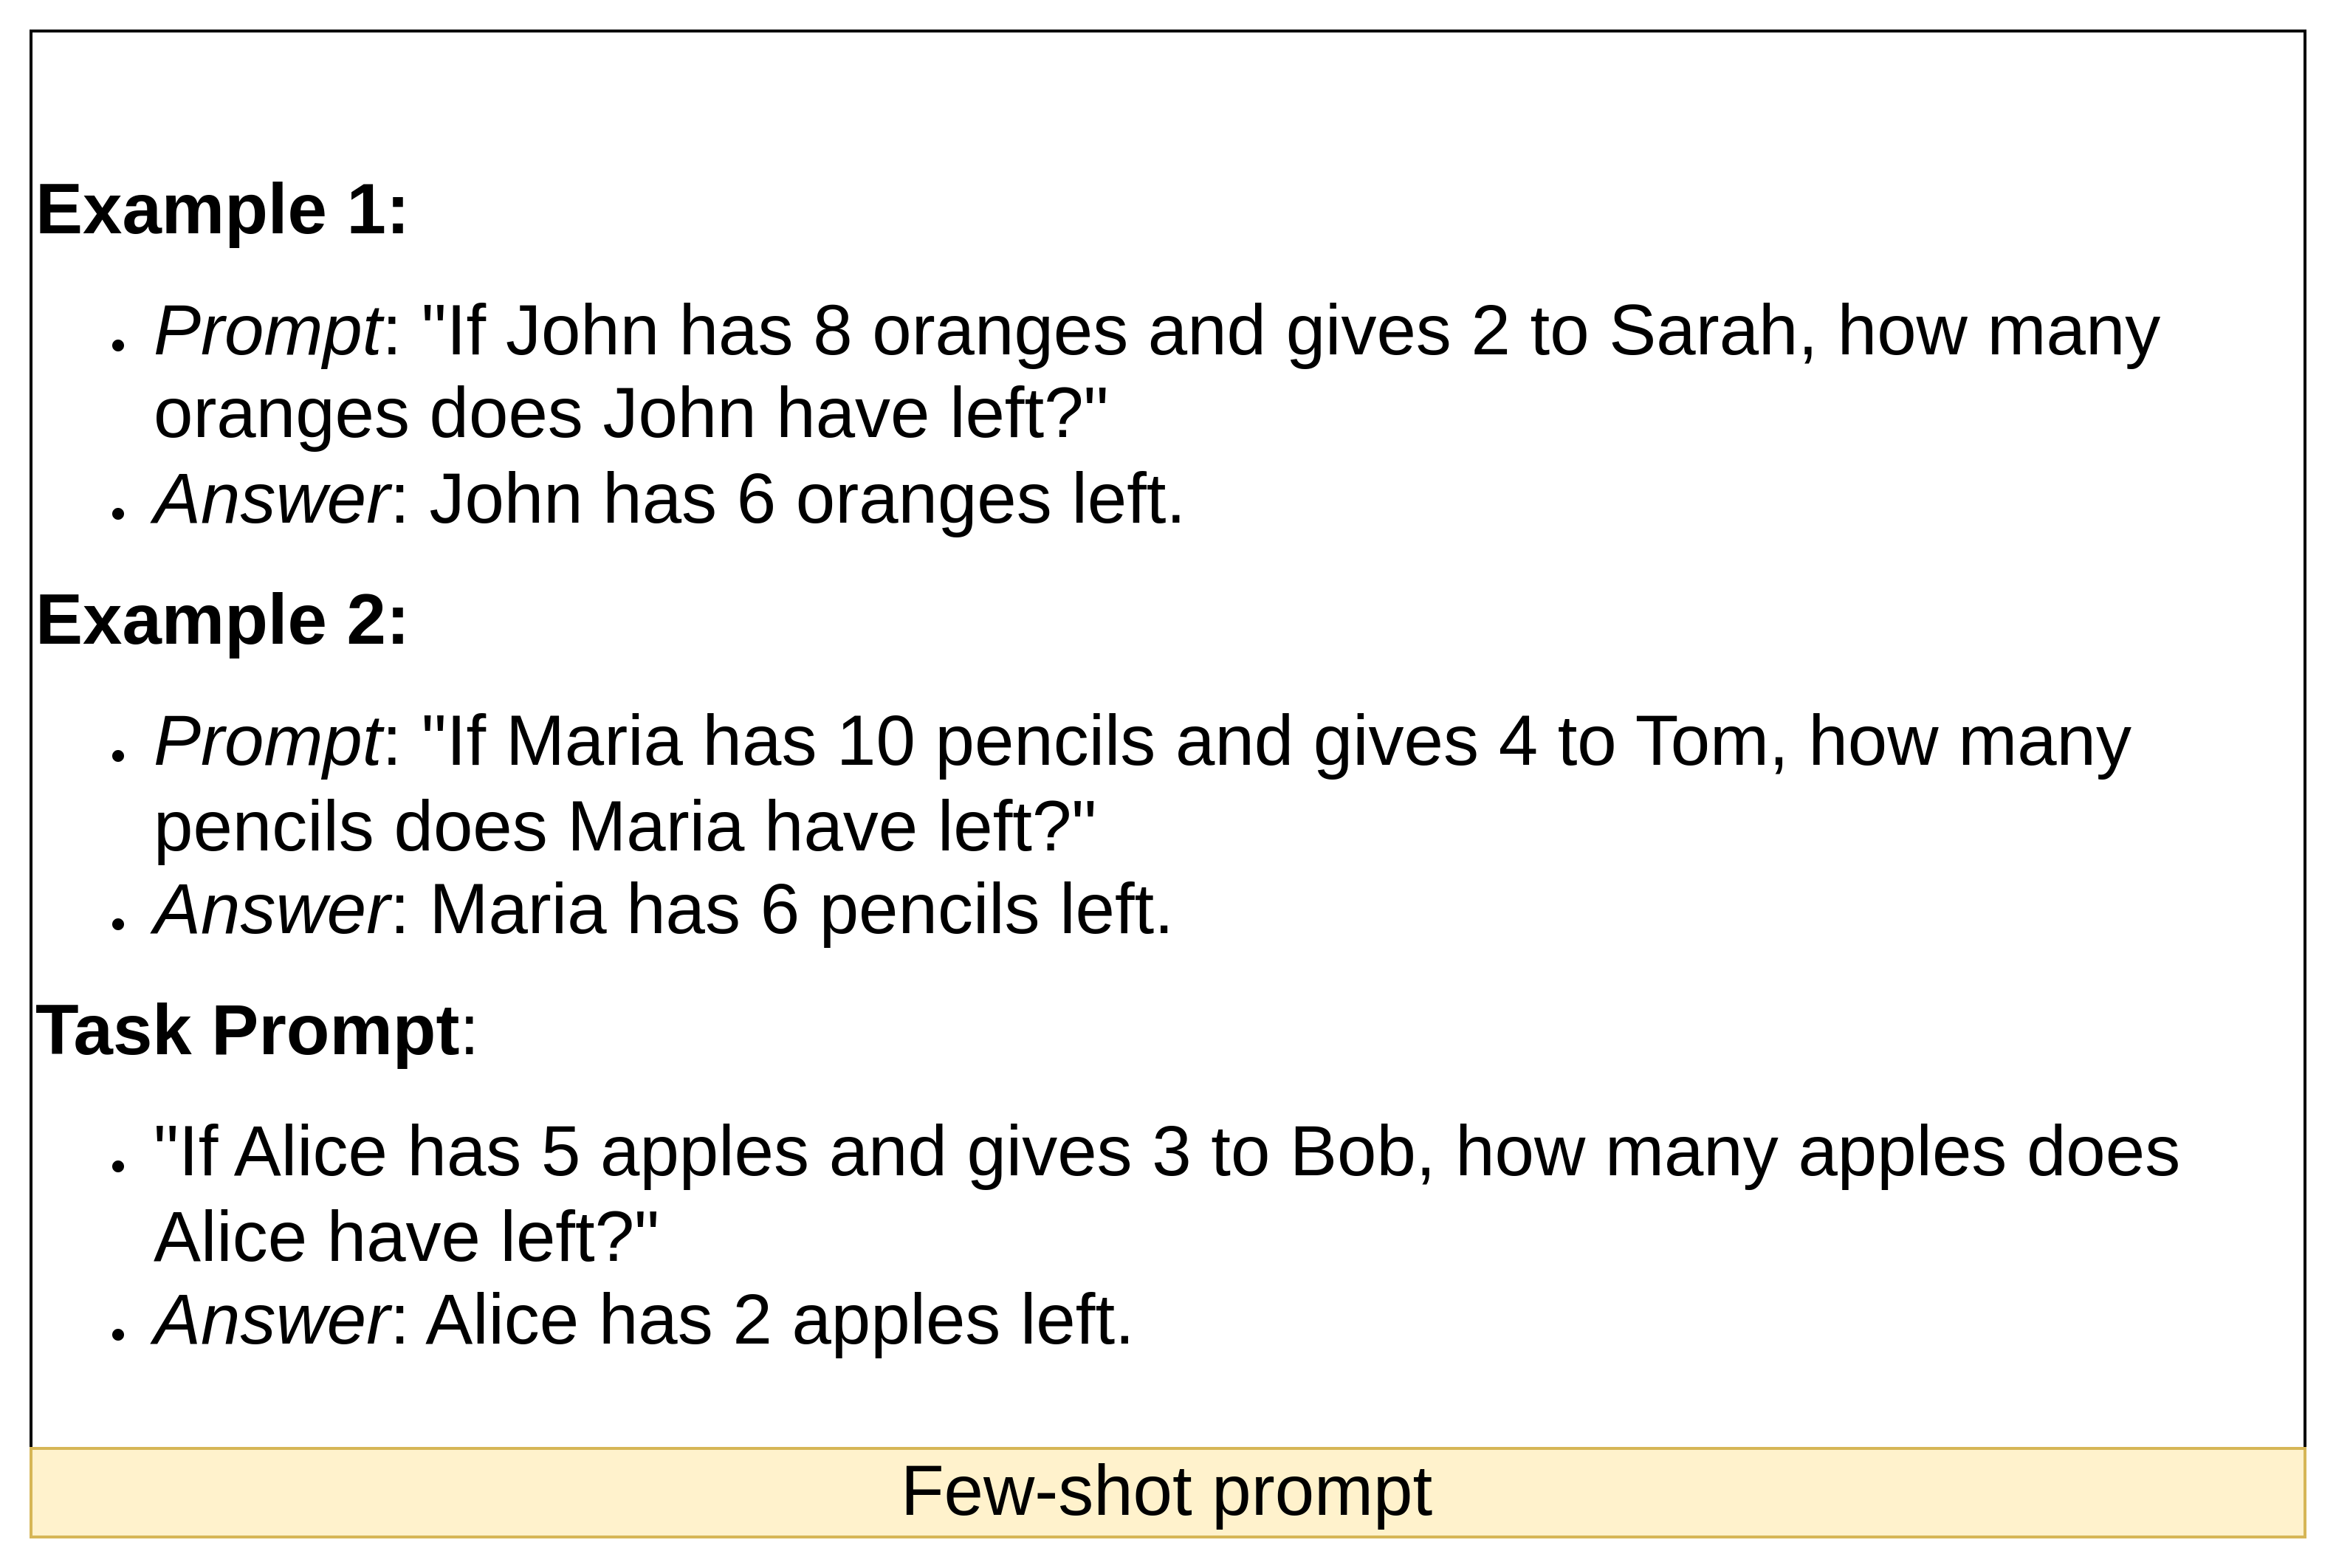
\includegraphics[height=2in]{./pics/soaPics/fewshotpromtexample.png}
			\caption{Few-shot prompt example}
			\label{fig:fewshotexample}
		\end{subfigure}%
		~ 
		\begin{subfigure}[t]{0.5\linewidth}
			%\centering
			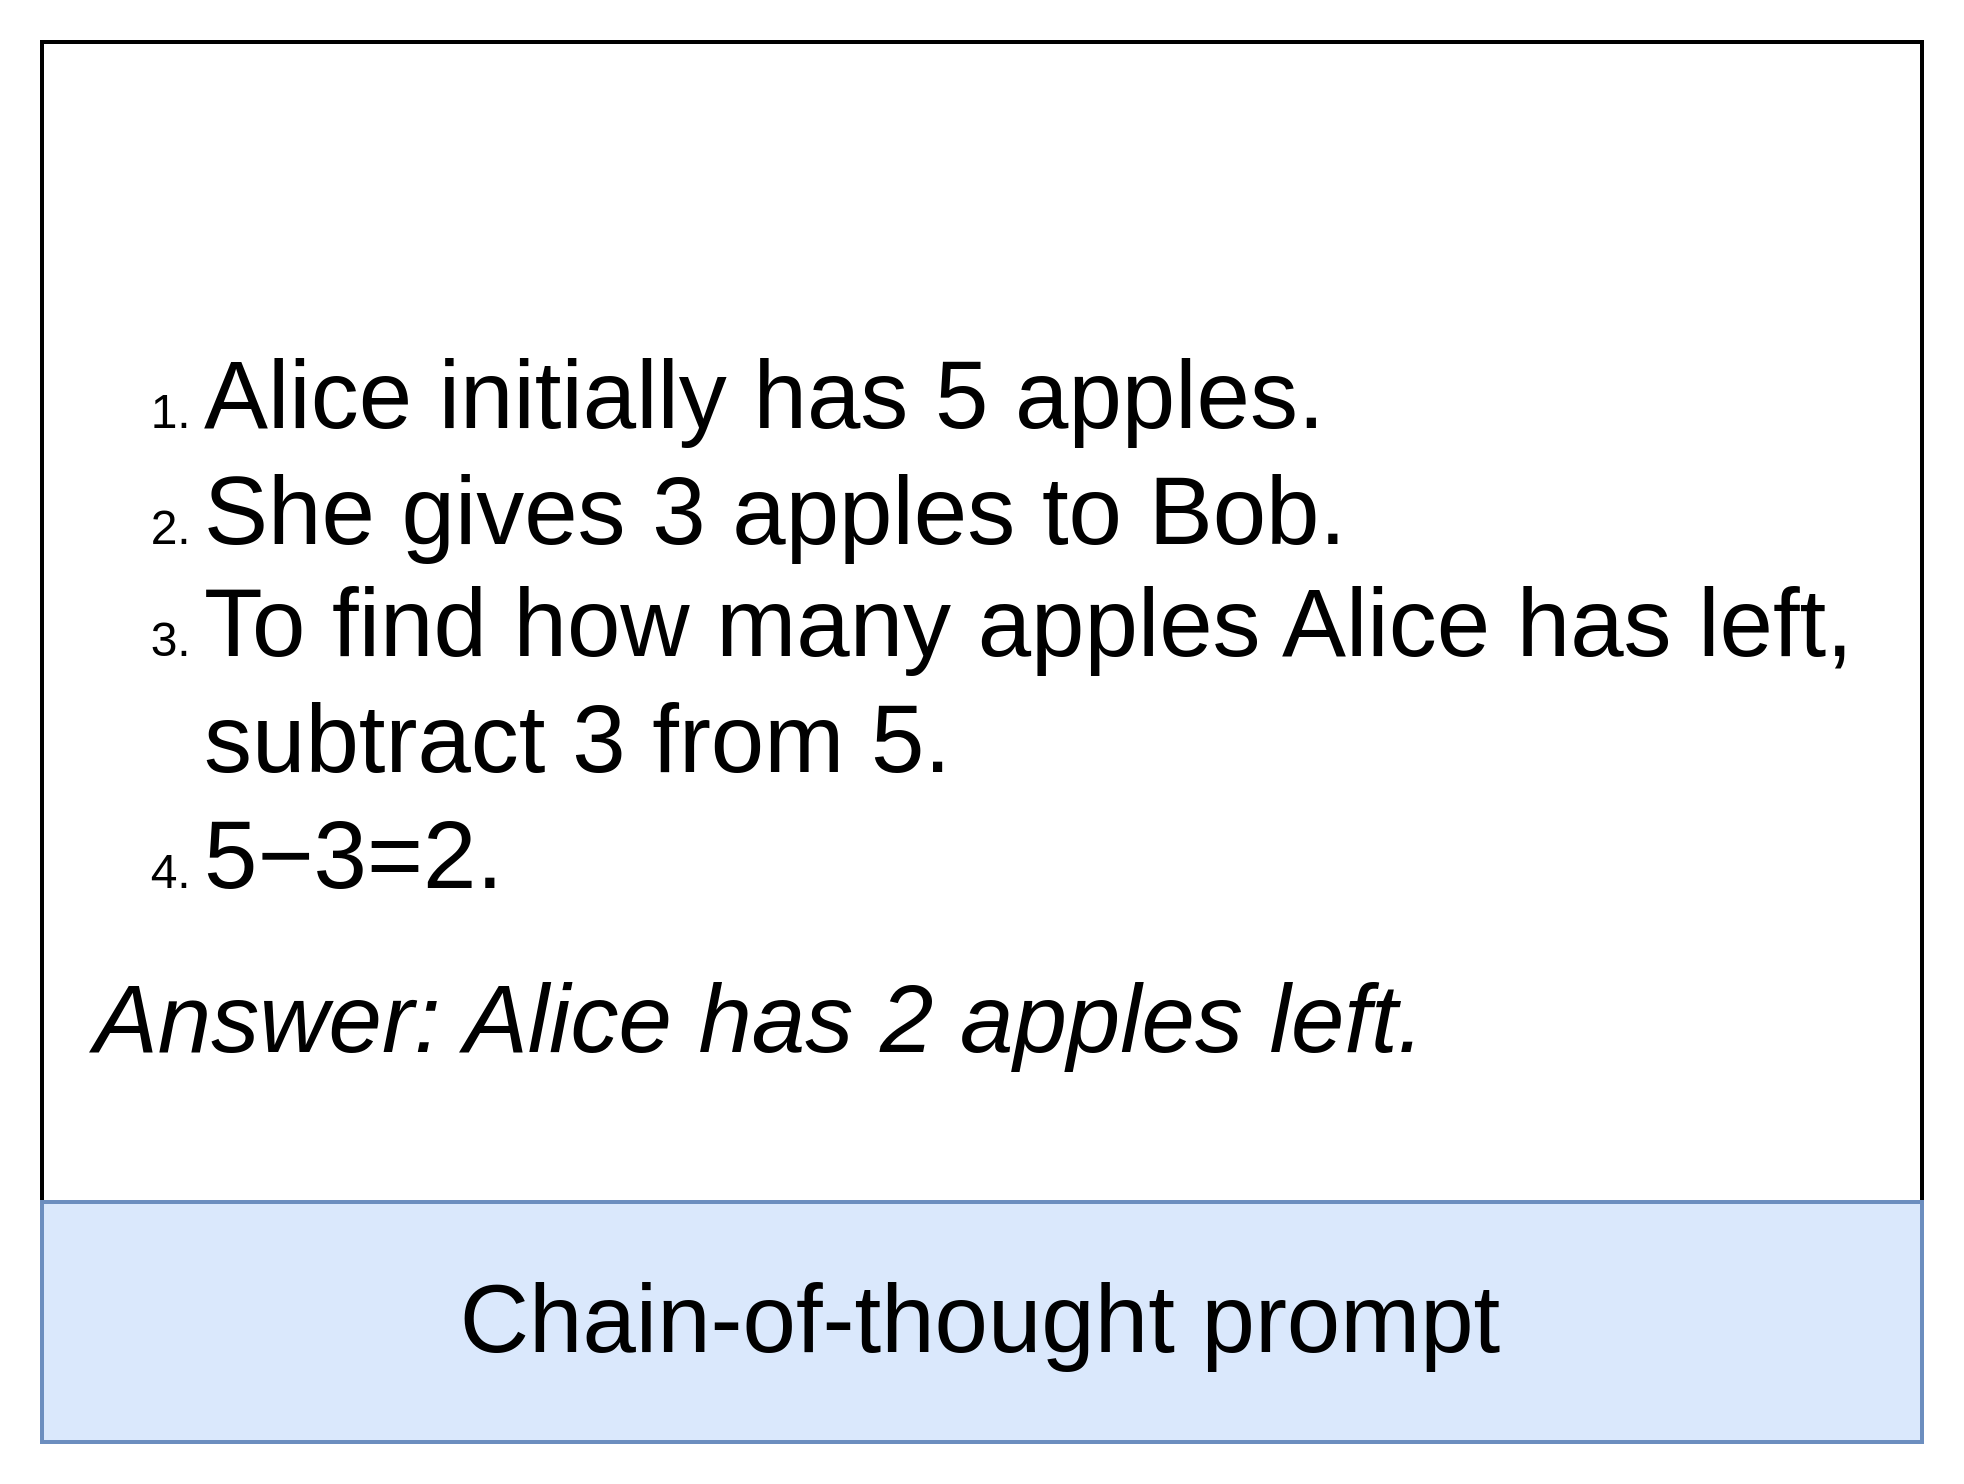
\includegraphics[height=2in]{ ./pics/soaPics/cotpromptexample.png }
		
			\caption{Chain-of-thought prompt example}
			\label{fig:cotexample}
		\end{subfigure}
	%	\label{fig:fewshotcotexample}
		\caption{ Few-shot vs Chain-of thought example }
	\end{figure*}
	
	
	
\end{itemize}
\section{Conclusion}
In this chapter, I provided the essential background for Model-Driven Engineering, covering key aspects such as metamodeling and its related artifacts, automation tasks, and the concept of co-evolution with the different concepts related to evolution. Additionally, an overview of Large Language Models was presented to highlight their relevance in this thesis. This foundation establishes the necessary understanding for the exploration of following chapters.

%definition
\chapter{State Of The Art}

\chaptermark{State Of The Art}
%offline and online process
In this chapter, I present an overview of what has been done in the field of Model-Driven Engineering in the context of code co-evolution. I split this overview into five  parts. In section \ref{changedetection}, I present the metamodel change detection approaches. Section \ref{coevolutionartifacts} presents the co-evolution of model, transformations, constraints with evolving metamodel. In section \ref{coevolutioncode}, I discuss code co-evolution and relevant literature about API-client evolution, and language evolution. In Section \ref{behavioralcorrectness}, I browse related work to checking the behavioral correctness of code co-evolution. Section \ref{llmsforcoevolution}, presents an overview of the use of LLMs in related MDE and SLE tasks. I finish this chapter with a discussion focused on limitations and research gap.
 \section{Metamodel change detection}
 \label{changedetection}
 One of the intrinsic properties of software artifacts is its continuous evolution~\cite{mens2008introduction}. Like any software artifact, metamodels are meant to evolve to meet the represented domain. %one key sentence of the context
 In this thesis, the context is triggered by the metamodel evolution, that's why I find essential to understand this evolution in detail.
 %metamodel diffing
 A lot of work has been done on metamodel diffing.
 Detection approaches can be classified into two main categories: online\footnote{Offline approaches perform detection after the metamodel has been evolved.} detection approaches, and offline\footnote{Online approaches perform instant detection for each change during the metamodel evolution} detection approaches. This classification can be refined using some factors as detailed by Hebig et al.~\cite{hebig2016approaches}: automation degree, types of detected changes, considered issues (overlap, indefinite length, hidden changes, order of changes, and undo operations)~\cite{hebig2016approaches}.
 	
 \begin{table}[p]
 	\centering
 	
 	\resizebox{16cm}{!} {
 		{\small
 			\begin{tabular}{l|c|c}%|l|l|l|l|l|l|l|}
 			%\hline
 			\toprule 
 			Type & group  & Change name  \\ \midrule
 			
 			\multicolumn{1}{l|}{ Atomic changes}
 			& \multirow{2}{*}{ \begin{tabular}[c]{@{}l@{}} Structural \\ Primitives\end{tabular} } 
 			&  \begin{tabular}[c]{@{}l@{}} Create Package, Delete Package, Create Class,\\Delete Class, Create Attribute, Create Reference,\\ Delete Feature,change type, Create Opposite Ref.,\\Delete Opposite Ref., Create Data Type, \\Delete Data Type, Create Enum, Delete Enum, \\Create Literal,Merge Literal  \end{tabular}
 			\\  \cmidrule{2-3} 
 			& \multirow{2}{*}{ \begin{tabular}[c]{@{}l@{}} Non Structural \\ primitives\end{tabular}} 
 			&  \begin{tabular}[c]{@{}l@{}} Rename, Change Package,Make Class\\ Abstract, Drop Class Abstract,\\ Add Super Type, Remove \\Super Type, Make Attr. Identifier,\\ Drop Attr. Identifier, Make Ref. Composite, \\Switch Ref. Composite, Make Ref. Opposite,\\ Drop Ref. Opposite  \end{tabular}
 			\\   \cmidrule{1-3} 
 			\multicolumn{1}{l|}{ Complex changes}
 			& \multirow{2}{*}{ \begin{tabular}[c]{@{}l@{}} Specialization / \\Generalization Operators\end{tabular} } 
 			&  \begin{tabular}[c]{@{}l@{}} Generalize Attribute, Specialize \\ Attribute, Generalize Reference, \\Specialize Reference, Specialize\\ Composite Ref. Generalize Super Type,\\ Specialize Super Type \end{tabular}
 			\\  \cmidrule{2-3} 
 			& \multirow{2}{*}{ \begin{tabular}[c]{@{}l@{}} Inheritance \\Operators
 			\end{tabular}} 
 			&  \begin{tabular}[c]{@{}l@{}}  Pull up Feature, Push down Feature,\\ Extract Super Class, Inline Super Class, \\Fold Super Class, Unfold Super Class,\\ Extract Sub Classn Inline Sub Class \end{tabular}
 			\\  \cmidrule{2-3} 
 			& \multirow{2}{*}{ \begin{tabular}[c]{@{}l@{}} Delegation\\ Operators\end{tabular}} 
 			&  \begin{tabular}[c]{@{}l@{}} Extract Class, Inline Class, Fold Class,\\ Unfold Class, Move Feature over Ref.,\\ Collect Feature over Ref.  \end{tabular}
 			
 			\\  \cmidrule{2-3} 
 			& \multirow{2}{*}{ \begin{tabular}[c]{@{}l@{}} Replacement\\ Operators\end{tabular}} 
 			&  \begin{tabular}[c]{@{}l@{}} Subclasses to Enum., Enum. to Subclasses,\\ Reference to Class, Class to Reference, \\Inheritance to Delegation, Delegation to Inheritance,\\ Reference to Identifier, Identifier to Reference \end{tabular}
 			\\  \cmidrule{2-3} 
 			& \multirow{2}{*}{ \begin{tabular}[c]{@{}l@{}}Merge /\\ Split Operators Merge\end{tabular}} 
 			&  \begin{tabular}[c]{@{}l@{}} Merge Features, Split Reference by Type,\\ Merge Classes, Split Class, Merge Enumerations\\\end{tabular}
 	\\
 	\\
 			\bottomrule
 			
 			% &  \cellcolor{CellColor1} \CIRCLE & \cellcolor{CellColor1}  &  \cellcolor{CellColor1}\CIRCLE & \cellcolor{CellColor1}\CIRCLE \\ \bottomrule
 		\end{tabular}
 	}
 }
 \caption{Catalog of model operators} 
 \label{table:changesCatalog}
 \end{table}
 %breaking not breaking?
 
  Furthermore, many of them classified the detected changes based on their impact on the treated artifact (e.g., models, constraint, transformation, and code). In Table~\ref{table:changesCatalog}, I put the largest set of changes types that I found in literature~\cite{herrmannsdoerfer_extensive_2011}. Later in Section \ref{sec: ap1_changedetection}, I specify the treated subset of these changes. 
  
  %with their possible impact on the code.
  In Model-Driven Engineering, depending on their impact on model instances, metamodel changes can be divided into three categories \cite{gruschko2007towards}:
 \begin{itemize}
 	
 	\item	Non-breaking changes that occur in the metamodel but do not break other artifacts of lower abstraction level.%can be resolved automatically.
 	\item Breaking and resolvable changes break the conformance of existing data, although they can be automatically adapted.
 	\item Breaking and unsolvable changes break the conformance of existing data, that cannot be automatically adapted, and require user intervention.
 \end{itemize}
 
 In API evolution similar context, API changes can be classified as non-breaking API changes or breaking API changes. A non-breaking change is backward compatible. This kind of changes aims to extend the functionalities or fix errors. A breaking change is not backward compatible. In this case, client code calling the evolved API by a breaking change fails to compile or may behave differently at runtime \cite{dig2006apis}.
 
 
 In literature, two types of evolution changes are considered when evolving a metamodel: \emph{atomic} and \emph{complex} changes~\cite{hebig2016approaches,Herrmannsdoerfer2011}. 
 Atomic changes are additions, removals, and updates of a metamodel element. Complex changes consist of a sequence of atomic changes combined together~\cite{vermolen_reconstructing_2012},~\cite{khelladi2015detecting}. For example, move property is a complex change. Where a property is moved from a source class to a target class. This complex change is composed of two atomic changes: delete property and add property~\cite{Herrmannsdoerfer2011}. 
 Many approaches exist to detect changes between two metamodel versions~\cite{Alter2015, williams2012searching,cicchetti_managing_2009,langer_posteriori_2013,vermolen_reconstructing_2012,Khelladi2016,bettini2022executable}.
%  \begin{table*}[t]
%  		\caption{Catalog of changes that occur during the metamodel evolution. (To fill)}
%  	\label{table:changesCatalog}
% \vspace{1em}
% 	\begin{tabular}{ |c|c|c| } 
% 	
% 		\hline
% 		Type & group  & Change name \\
% 		\hline
% 		\multirow{4}{4em}{ Atomic changes} & Delete class  \\ 
% 		& Delete property \\ 
% 		& Add class \\ 
% 		& Add property \\ 
% 		& Rename class \\ 
% 		& Rename property \\ 
% 		& Generalize property \\ 
% 		\hline
% 		\hline
% 		\multirow{5}{4em}{Complex changes} & Move property \\ 
% 		& Push property  \\ 
% 		& Pull property\\ 
% 		& Inline class\\
% 		& Change property type\\
% 		\hline
% 		
% 	\end{tabular}
% 	\end{table*}
% 	\vspace{1em}
% 	
 	
 	  
 
 				

 	
 	

%TODO Discussion part 

%operation-base ?difference-based

Demuth et al. \cite{demuth2015constraint}, Herrmannsdoerfer et al. \cite{herrmannsdoerfer2009cope}, Khelladi et al. \cite{khelladi2016detecting} are online approaches that take into consideration undo operations while the metamodel evolution.
In contrast, other approaches \cite{williams2012searching,10.1145/2000410.2000416,levendovszky2014semi,garces2009managing,cicchetti_managing_2009,langer_posteriori_2013,garcia2012model,xing2006refactoring,moghadam2012automated,vermolen_reconstructing_2012} adopt offline detection method. However,  offline detection may cause an order issue, particularly in \cite{williams2012searching,10.1145/2000410.2000416,levendovszky2014semi,garces2009managing,langer_posteriori_2013,garcia2012model,xing2006refactoring,moghadam2012automated}. Notably, none of these approaches consider hidden changes, with the exception of Vermolen et al.~[57].


Regarding to the automation degree of the approaches, Herrmannsdoerfer et al. \cite{herrmannsdoerfer2009cope} and
Williams et al. \cite{williams2012searching} are manual methos. Di Ruscio et al. \cite{10.1145/2000410.2000416}, Vermolen et al. \cite{vermolen_reconstructing_2012}, and Khelladi et al. \cite{khelladi2016detecting} are all semi-automatic that require user decision to select final output changes.
Demuth et al. \cite{demuth2015constraint}; Levendovszky \cite{levendovszky2014semi},Cicchetti et al. \cite{cicchetti_managing_2009}, Garces et al. \cite{garces2009managing}, Langer et al.~\cite{langer_posteriori_2013}, Garcia \cite{garcia2012model}, Xing  et al. \cite{xing2006refactoring}, Moghadam et al. \cite{moghadam2012automated} are full automatic approaches.




Moghadam \cite{moghadam2012automated}, Vermolen \cite{vermolen_reconstructing_2012} and \cite{khelladi2016detecting} take into consideration indefinite length of a complex change.
Khelladi et al. \cite{khelladi2016detecting} take into consideration overlap issue.


%Structural Changes: Additions, deletions, or modifications to classes, attributes, associations, or inheritance structures.
%Semantics or Behavioral Changes: Modifications in the constraints, rules, or behavior definitions in the metamodel.
All these approaches propose structural changes detection: additions, deletions, or modifications to classes, attributes, associations, or inheritance structures \cite{10.1007/s10270-013-0392-y}. When a metamodel is defined, the definition of the structural side of the representation of a domain is given. The behavioral side is given through constraints \cite{10.1007/s10515-009-0053-0}. In this thesis, I focus only on the structural metamodel changes, any change occurring on behavioral aspects of a language, at metamodel level, is out of the scope of this dissertation.
%Following this definition, in this section, I give the structural changes. Another usage ? behavioral impact ? structural impact? structural error ? behavioral error? static/ runtime? 
%TODO  put this in a conclusion of the chapter?
After studying the literature change detection approaches of metamodel, relatively to the challenges that I discussed in the challenges section \ref{challenges}, I found that Khelladi et al. \cite{khelladi2016detecting} handle a large set of changes. Furthermore, their approach handle all the issues that I mentioned. 
It is a semi-automatic approach but this adds a trust value to the approach because automatic approach may have order or overlap issues.

Another reason to choose Khelladi et al. \cite{khelladi2016detecting} approach is their output representation and vocabulary. It required a minimum effort of adaptation because I use the same changes representation (more detail in Section \ref{??}).

%The usage of Khelladi et al. \cite{khelladi2016detecting} in my work is explained in section??

 \section{Co-evolution of models, constraints, and transformation}
 \label{coevolutionartifacts}
% In MDE ecosystem, the metamodel is the starting point to have other artifacts that we defined in section ?.
  In this section, I will present an overview of the existing work about these artifacts co-evolution. Note that if the solution is applied during the evolution of the metamodel, we call it an online solution, otherwise it is offline.
 The comparison, advantages, and drawbacks of the presented approaches is out of the scope of this dissertation.
 
\subsection{Metamodel and model co-evolution}
Due to metamodel evolution, instance models become no conformant. A set of resolutions are applied to co-evolve the models to gain again the conformity to the metamodel.
 %  - COPE - Automating Coupled Evolution of Metamodels and Models : couple evolution co-evolution
Two strategies to evolve models due to metamodel evolution. 
In the first strategy, the metamodel is the artifact to be adapted in a way that the old models can still be used with the evolved modeling language without adapting the models \cite{herrmannsdoerfer2009cope}. This approach suggest the resilience of the models. The second strategy adapts the metamodel in a breaking manner for the models, that must be adapted by transforming them into a new version that conforms to the adapted metamodel.

%change order, resolution order
%Once the metamodel changes are detected, using one of the previously presented approaches in Section ?, 
 %a set of resolutions are applied to co-evolve the model to gain again the conformity to the metamodel.
 %change order, resolution order
 The co-evolution between metamodel and models can be processed manually, but it requires a huge expertise, and when the number of models to co-evolve increases, manual co-evolution becomes hard task. 
 Most of automatic and semi-automatic co-evolution approaches use automatic or manual diffing metamodel approaches in their solutions. Model co-evolution approaches that exist can be categorized into five categories \cite{Hebig2017}. The first category is Resolution Strategy Languages that specify in a transformation language how to update the model given the list of metamodel changes \cite{10.1007/978-3-540-87875-9_44,sprinkle2004domain,wimmer2010using,10.1007/978-3-642-30476-7_13,10.1007/978-3-642-38883-5_10,10.1007/s10270-012-0313-5,10.1007/s10270-012-0296-2}. The category Resolution Strategy Generation groups approaches that generate full or partial resolution for each metamodel change \cite{del2007semi,de2008generating,garces2009managing,meyers2011generic,anguel2014using}.
 
 
 The third group of Predefined Resolution Strategies contains approaches that provide automation, when it is possible, by applying predefined resolution strategies \cite{hossler2005coevolution,florez2012coevolution,fernandez2013adapting,wachsmuth2007metamodel,cicchetti2009managing,van2011generic,becker2007process,herrmannsdoerfer2009operation,wittern2013determining}. 
 
 %We find three categories of metamodel and model co-evolution approaches.% Approaches based on resolution strategy languages that propose transformation languages created given the metamodel changes. The second category groups Resolution strategy generation approaches that allow to generate full or partial resolutions for each metamodel change.
 
  Some of these approaches require user intervention to make decision on the selected operation to adapt the model.
  The fourth category of Resolution Strategy Learning that adopts machine learning algorithm to select the resolution strategy for metamodel changes.\cite{anguel2013towards}.%TODO Look for full paper
 
The fifth and last category is called Constrained Model Search approaches. It groups approaches that do not use the metamodel changes, but use the original model and the new metamodel to apply a constrained-based search of valid model variants \cite{demuth2016co,gomez2014approach,schonbock2014care}. Other approaches consider the model co-evolution problem as an optimization one that does not need the list of changes of the metamodel \cite{kessentini2016automated,kessentini2019automated,kessentini2020interactive}.
%Demuth el al. [6] who used it for models co-evolution.
% There are also approaches for semi-automatic co-evolution of models that rzquires the user intervention to make decision on the selected operation to adapt the model.

%The point is that for metamodel and model co-evolution; predefined approaches exist, full automatic approaches exist to put in the discussion


%For example, when a type restriction is applied to a property in a metamodel, the generic solution implemented in the approaches of Meyers et al. and Edapt would delete prop- erty instances that are no longer conform. In contrast, the approach of Wachsmuth would allow the user to specify a type conversion. Thus, due to giving additional control to the user, the property values can be preserved in the mod- els. Consequently, if there is the need for an outcome that deviates from generic solutions, approaches are required to provide the user with a certain amount of control about the results of the resolution

Depending on whether a user intervention is needed or not to apply predefined or generated resolutions, there are automatic and semi-automatic approaches.
In one hand, Di Ruscio et al.~\cite{10.1007/978-3-642-33654-62}, Levendovszky et al.~\cite{levendovszky2014semi}, Anguel et al.~\cite{anguel2013towards,anguel2014using}, Cicchetti et al.~\cite{cicchetti2008automating}, van den Brand et al.~\cite{van2011generic}, are automatic model co-evolution approaches.

%Di Ruscio et al. \cite{10.1007/978-3-642-33654-62}, MCL Levendovszky et al. \cite{levendovszky2014semi}, Anguel et al. \cite{anguel2014using},cicchetti et al. \cite{cicchetti2008automating}, van den Brand et al. \cite{van2011generic}, CBRMig~\cite{anguel2013towards} are automatic model co-evolution approaches.

In another hand, semi-automatic approaches that I found in literature are: de Geestwe et al.~\cite{de2008generating},  Garcès et al.~\cite{garces2014adapting}, Wittern et al.~\cite{wittern2013determining} (for atomic changes, the co-evolution is automatic, for complex changes, the co-evolution is manual).

%semi-automatic vs automatic : trade-off between desired correctness of the resulting models and automation that khelladi survey cite an example of a property type restriction. Some approaches would delete the property instances that are no longer conform where other approaches propose a type conversion. 

Related to the previous section \ref{changedetection}, some model co-evolution approaches were interested in studying the impact of metamodel evolution on models.
COPE~\cite{herrmannsdoerfer2009cope}, Wachsmuth et al.~\cite{wachsmuth2007metamodel}, and Kessentini et al.~\cite{kessentini2018integrating,kessentini2020interactive} do not explicitly study the impact of metamodel evolution on  models.
 
 Cicchetti et al.~\cite{cicchetti2008automating} categorize metamodel modifications  into additive, subtractive, and updative. Their approach starts by generating a difference model, then a transformation model to co-evolve models, without a step dedicated impact analysis.
Garcès et al.~\cite{garces2009managing} computes equivalences and differences between any pair of metamodels, simple and complex changes. These equivalences and differences are then represented as matching model. In the second step, the matching model is translated into an adaptation transformation by using a Higher-Order Transformation (HOT) that is later executed. A matching model is used to generate a transformation model but no explicit analysis for the impact of metamodel evolution on the models.

I found that only Demuth et al.~\cite{demuth2016co} studied the impact of metamodel evolution on models. Their consistent change propagation focuses on maintaining consistency between artifacts using constraints (metamodel itself and existing models). Later, the impacted constraints are used to propose repairs, then manual intervention is needed to select and apply these repairs.

 

%\cite{kessentini2018integrating,kessentini2019automated,cicchetti2008automating,herrmannsdoerfer2009cope,garces2009managing,wachsmuth2007metamodel},
\subsection{Metamodel and constraints co-evolution}
Another artifact that depends on the metamodel and needs to be adapted as the metamodel evolves is constraints.
 Constraints co-evolutions that exist in literature may be online \footnote{Online approaches perform instant co-evolution for each change during the metamodel evolution} or offline \footnote{Offline approaches perform co-evolution after the metamodel has been evolved.}. Every approach has its own co-evolution mechanism that treats specific types of metamodel changes and has its automation degree. Demuth et al. \cite{10.1007/978-3-642-41533-3_18} propose a template-based of the predefined structure of the updated constraint taking into consideration few change types. Markovich et al.~\cite{markovic2008refactoring} propose refactoring rules that depend on the impact of UML class diagram evolution on the constraints. In this approach, the user selects the refactoring rule to be applied on the model then on the depending constraints. Another constraints co-evolution approach is METAEVOL proposed by Hassam et al. \cite{hassam2011assistance}. METAEVOL is a tool based on a transformation language. Kusel et al.~\cite{kusel2014systematic} propose a solution for the co-evolution of the constraint body and do not include its context that may need to be co-evolved also.
 Cabot et al.~\cite{cabot2004automatic} treat OCL constraints co-evolution due to metamodel deletion change. Khelladi et al.~\cite{khelladi2017semi} propose an approach that records the metamodel atomic and complex changes in a chronological order, then apply one or many resolutions to co-evolve the constraints. Batot et al.~\cite{8101267} tackle the constraint co-evolution problem as a multi-objective optimization problem. They apply heuristic-based recommendation approach that does not use a predefined set of transformation rules to co-evolve the constraints.
 
 
 Cherfa et al. \cite{cherfa2021identifying} provide an assistance to developers working on OCL constraint co-evolution, by focusing on the structures in the metamodel that potentially cause problems and which ones need new OCL constraints (after the co-evolution). Their approach does no explicitly process an impact analysis.%instead of exploring the solution domain (generating the missing constraints), /
 %Since the set of constraints (F) is incomplete and hence does not cover all the concepts of the new metamodel version, a set of MIS that can arise from the evolution operators. implies the designer  in treating these mis.
 
% Describe what have been done in analysing the impact of metamodel evoluitoon on the constraits , and how the co-evolutinon correctness is checked becausie constrains are behavioral description of the metamodel.
 Regarding the impact analysis of the metamodel evolution, Kusel et al.~\cite{kusel2014systematic} study this impact on OCL expressions. They distinguished between breaking and non-breaking impact. Moreover, they divided the changes into three groups: constructive changes which are non-breaking where destructive changes and updative changes which are considered breaking changes if they have at least one breaking impact case on the constraints. Furthermore, their study includes %a table that contains
  every possible case and the corresponding resolution. This paper~\cite{kusel2014systematic} proposes syntactic co-evolution that can be checked by a compiler, where the semantic co-evolution correctness is checked through Pattern-based formal specification Modeling Language for Model Transformations (PaMoMo)~\cite{10.1007/s10515-012-0102-y}. The correctness checking process uses a set of Pamomo specifications (input models) to be verified before and after OCL expressions' co-evolution.
  % Pamomo states. properties the models must fulfill

In their co-evolution approach, Batot et al.~\cite{batot2017heuristic} first register metamodel elements that were deleted, added, or had their multiplicity changed between the two versions. %Computing atomic differences does; but does not require high level changes identification. 
 Then,they apply an NSGA-II heuristic algorithm to satisfy the objective functions. However, no additional correctness checking are performed. Finally, a syntactic comparison is processed to determine if a candidate constraint is the same as the expected one. Notably, the impact of metamodel evolution on OCL constraints is not explicitly analyzed.
  
   
  
 
%impact analysys: 
Hassam et al.~\cite{hassam2011assistance} proceed by a partial impact analysis, through a table that contains constraints context that is linked with the involved elements of the metamodel that is evolved. The designer is then, responsible to check the validity of the constraint. 

Khelladi et al.~\cite{khelladi2017semi} associate each evolved metamodel element to impacted constraint (context and body)  and precise the impacted constraint astnodes. However, no further correctness checking of their output.

%Other approaches do not study the impact of metamodel evolution on the constraint artifact like Batot et al. \cite{8101267}.

Cabot et al.~\cite{cabot2004automatic} as an impact analysis, identify the elements to be deleted (those selected by the user plus all the elements affected by them).

Regarding the automation degree of the approaches above, Demuth et al., Markovitch et al., and Cabot et al. \cite{10.1007/978-3-642-41533-3_18,markovic2008refactoring,cabot2004automatic}  approaches are fully automatic while Hassam, kusel and Khelladi, and Batot \cite{hassam2011assistance,kusel2014systematic,khelladi2017semi,8101267} propose semi-automatic approaches since the user must select from the recommended output constraints. 
\subsection{Metamodel and transformations co-evolution}

Almost all the existing transformation approaches that I find in literature have the same strategy. This strategy consists of evolving the impacted parts in the transformations in a semi-automatic manner requiring a human intervention. 
%start by analyzing the impact of the metamodel on the model transformations.
Garcia et al.~\cite{garcia2012model} proposed an ATL rule-based approach. This approach only guarantees that the evolved transformations are syntactically correct, but does not process any other correctness checking, including semantic correctness. % is not taken into consideration.
  Kusel et al.~\cite{kusel2015consistent} explained explicitly that his approach verifies semantic correctness through a set of properties expressed in PaMoMo language~\cite{10.1007/s10515-012-0102-y} as a kind of regression testing.

The approach of Khelladi et al.~\cite{khelladi2018change} covers the largest set of existing resolutions. In their change propagation-based approach, they allow to compose existing resolutions into a new one. This approach~\cite{khelladi2018change} does not process any semantic verification of the transformation co-evolution alongside the comparison with their ground of truth. Ruscio et al.~\cite{di2011needed} with their EMFMigraite tool, estimate first the cost of the co-evolution to decide about the co-evolution. EMFMigrate further explores the variability and common aspects of the co-evolution related to different type of artifacts. Moreover, they allow developers to manually replace or refine a resolution. All these approaches propose a unique resolution to co-evolve each transformation. Mendez et al.~\cite{mendez2010towards} study the relation between the metamodel and the transformations. It detects the transformations' inconsistencies after the metamodel co-evolution. then, depending on the impacting metamodel change, a resolution is suggested.
Garcés et al.~\cite{garces2014adapting} propose a solution based on adaptation chains via composition functions depending on the impacting metamodel changes.
Kessentini et al.~\cite{kessentini2018automated} followed a different approach that does not use the changes of the metamodel as input and does not process an impact analysis, but rather uses a search-based approach that relied on multi-objective heuristic algorithm NSGA-II. This approach has an objective function to minimize the number of errors of non-conformance between the metamodels and transformations. These errors can be statically detected by static semantic constraints. However, no semantic verification of the co-evolution correctness is processed.


% kusel2015consistent: formal specification language to describe correct- ness requirements for transformations (cf. [7] for details). A PaMoMo specification consists of declarative visual patterns, which may be positive, i.e., describing necessary conditions to occur (denoted by a “P”), or negative, which state forbidden situations (denoted by an “N”). Patterns are composed of two compartments containing object graphs typed on the source MM (left compartment) or target MM (right compartment). Objects in the source and target compartments may have attributes that may be assigned either a concrete value or a variable. A variable may be assigned to several attributes to ensure equality of their values. The specified patterns provide a well-defined operational semantics on basis of QVT- Relations [17], which allows to check whether pairs of input models and resulting output models fulfill the specified cor- rectness requirements, which in consequence allows to evalu- ate the semantic correctness of a transformation definition

Mendez et al.~\cite{mendez2010towards}, Garcés et al.~\cite{garces2014adapting}, and Ruscio et al. \cite{di2011needed} do not include any impact analysis of metamodel evolution on the transformations to be co-evolved. However, Garcès et al.~\cite{garces2014adapting} explains the impact of the evolution of the metamodel on the transformations through a motivating example but not an explicit study independent from the example. 
I found that only Mendez et al.~\cite{mendez2010towards} and Khelladi et al.~\cite{khelladi2018change} dedicated a detailed part in their approaches for the analysis of the impact of metamodel evolution on the transformations.
%All these approaches are semi-automatic methods,.

%mendez semi, khelladi semi, garces semi, ruscio semi,% partially atuomatically
Even though I consider the co-evolution in a larger scope in Model-Driven Engineering, my main focus is given to the co-evolution of the code that I detail in next section.

%\section{Software evolution}

 \section{Code co-evolution}
 \label{coevolutioncode}
 I divided the related work to code co-evolution  into four (4) main categories : 1) Metamodel and code co-evolution, 2) API and client code co-evolution, 3) Automatic Program repair, and 4) Consistency checking. 
 \subsection{Metamodel and code co-evolution}
 %by the fact that the code and other artefacts (models, constraints, etc) are on different levels of asbtractions In fact, the models and constriats are on closer level of abstraction of the metamodel, where each metamodel element is directly referenced/present in the depending artefacts.However, the code is on a lower level of abstraction where each  metamolde element has differents representation in the code.Thus One change in a ..... will affect n .....
 %TODO
 % artifacts are not executable code exctuable, checking fo the correctness impact on the overal system
 Co-evolution of code is distinguished from the co-evolution of other artifacts. This distinction is due to the fact that the code and other artifacts (models, constraints, transformations) are on different levels of abstraction. In fact, the models and constraints are on closer level of abstraction of the metamodel, where each metamodel element is directly referenced/present in the depending artifacts. However, the code is on a lower level of abstraction where each  metamodel element has different representation in the code. Thus $one$ change in a metamodel element will affect $n$ different code elements, in contrast to a $one$ to $one$ impact relationship between metamodel elements and models, constraints and transformation elements~\cite{kessentini2018integrating,kessentini2019automated,cicchetti2008automating,herrmannsdoerfer2009cope,garces2009managing,wachsmuth2007metamodel,batot2017heuristic,khelladi2017semi,correa2007refactoring,kessentini2018automated,khelladi2018change,garces2014adapting,10.1007/978-3-642-36089-3_9,kusel2015consistent,kusel2015systematic}.
 
 Yu et al.~\cite{yu2012maintaining} propose to co-evolve the metamodels and the generated API in both directions. However, they do not co-evolve the code on top of this generated API.
  % which our approach does. 
 %
  Khelladi et al.~\cite{Khelladi2020} propose an approach that propagates metamodel changes in the code as co-evolution mechanism. Nonetheless, it is based on static analysis to detect the impacts and not on the actual errors that appear from the compilation of the code after the metamodel evolution. It further applies a semi-automatic co-evolution requiring developers' intervention, and without checking behavioral correctness with tests or any comparison to a baseline. 
 
 
 %%%%%%%%%%%%%%%%%%%%%%%%%%%%%%%%%%%%%%%%%%%%%%%%%%%%%%%%%%%%%%%%%%%%%%%%%%%%%%%%%%%%%%
 \subsection{API and client code co-evolution}
 \label{API_evolution}
 
 %In this paper, we focus so far the co-evolution on the direction metamodel to code, which is not trivial. 
 
 Existing approaches for code migration, whether library code or API calls, are related to our work. % We focus on the main existing approaches to compare them with our approach.
   Henkel et al.~\cite{henkel2005catchup} propose an approach whose implementation is called CatchUp!. It captures refactoring actions of the library and replays them on the code to migrate. However, they support limited types of changes as renaming, moving, and class type changes. 
 
 Nguyen et al. \cite{nguyen2010graph} also propose an approach that guides developers in adapting code by learning adaptation patterns from previously migrated code. Similarly, Dagenais et al.~\cite{dagenais2011recommending,5070565,10.1145/1932682.1869486} also use a recommendation mechanism of code changes by mining them from previously migrated code. 
 %
 Anderson et al.~\cite{andersen2010generic} proposed to migrate drivers in response to evolutions in Linux internal libraries. It identifies common changes made in a set of files to extract a generic patch that can be reused on other code parts. Gerasimou et al.~\cite{10.1145/3194793.3194798} extract a set of mapping rules and apply code-based transformations to update its clients.
 
 % Survey about Library evolution \cite{10043250}
 
 Zaitsev et al.~\cite{10043250} present a survey about library evolution, that involves developers from two industrial companies: Arolla and Berger-Levrault in a hand, and Pharo as an Open-Source Community in another hand. In this survey, the study was conducted in both perspectives: client side and library side. Kula et al.~\cite{10.1016/j.infsof.2017.09.007} studied from library side, the impact of refactoring activities on evolving client-used APIs.
 Other works focused on the client side and how do client applications' developers react to the evolution of the libraries they depend on~\cite{10.1145/2393596.2393662,7332471,7816485,7884616,10.1007/s11219-016-9344-4,10.1007/s10664-017-9521-5}. Jezek et al. \cite{10.1016/j.infsof.2015.02.014} treat both client and library perspectives. They studied the compatibility aspect of the APIs and the impacts of the library evolution on the programs using it. Further detail about the supporting library update can be found in the PhD thesis of Zaitsev Oleksandr~\cite{zaytsev:tel-03998632}. Shaikh et al.~\cite{10.1145/3092703.3092721} studied Behavioral Backward Incompatibilities. In their paper, they process a cross-version regression testing to understand the behavioral changes of APIs during evolution of software libraries.

 %ref :Automatically Generating Refactorings to Support API Evolution
% ref :Experience Paper: A Study on Behavioral Backward Incompatibilities of Java Software Libraries
 
% 

\begin{table*}[t]
\centering
\caption{Related work comparison (to position )} 
\label{table:relatedWorkTable}
	\resizebox{16cm}{!} 
{\normalsize
\begin{tabular}{l|l|l|c|c|c|c}%|l|l|l|l|l|l|l|}
%\hline
\toprule 
 Approaches &Category & Approach & Automation & \begin{tabular}[c]{@{}c@{}}Requires \\ pre-learning\end{tabular}& Change types & Validation  \\ \midrule
 
\multicolumn{1}{l|}{ \textbf{Lamothe et al. \cite{9079197}}} & \multirow{2}{*}{} & \multirow{3}{*}{} &Semi-automatic &Yes $\checkmark$  &  \begin{tabular}[c]{@{}l@{}} Encapsulate, Move method,Remove parameter,\\Rename, Consolidate, expose implementation,\\ add contextual data,change type,\\ Replaced by exeternal API  \end{tabular}  & No $\times$  \\ \cmidrule{1-1} \cmidrule{4-7} 

\multicolumn{1}{l|}{\textbf{Fazzini et al. \cite{10.1145/3387905.3388608}} } &   \begin{tabular}[c]{@{}l@{}}Android api \\migration\end{tabular} &    \begin{tabular}[c]{@{}l@{}} Identifying migration patterns and \\rank them to select the most context-similar  \end{tabular}    & Fully-automatic& Yes $\checkmark$    &\begin{tabular}[c]{@{}l@{}}Any change in AST level\\ ( Insert/Move/Update/Delete)\end{tabular} &Yes $\checkmark$  \\ \cmidrule{1-2} \cmidrule{4-7} 

\multicolumn{1}{l|}{\textbf{Meng et al. \cite{10.5555/2486788.2486855}}} &   \begin{tabular}[c]{@{}l@{}}Bug fix \\context \end{tabular}              &          &  Semi-automatic& Yes $\checkmark$   & \begin{tabular}[c]{@{}l@{}}Any change in AST level\\ ( Insert/Move/Update/Delete)\end{tabular}& No $\times$ \\ \midrule

\multicolumn{1}{l|}{ \textbf{ Wu et al. \cite{6062100}}} & \multirow{4}{*}{} &    \begin{tabular}[c]{@{}l@{}} Hybrid approach using call \\ dependency graph and textual similarity   \end{tabular}                 
& Semi-automatic
&No $\times$ 
&\begin{tabular}[c]{@{}l@{}} change rules  :\\ One-to-One, One-to-Many \\ Many-to-One, Simple-Deleted  \end{tabular}      
& No $\times$ \\ \cmidrule{1-1} \cmidrule{3-7} 

\multicolumn{1}{l|}{\textbf{ Dagenais et al. \cite{dagenais2011recommending,5070565}}} 
&                   
&  \begin{tabular}[c]{@{}l@{}}     Recommendation approach for \\ compilation errors' correction     \end{tabular}            
& Semi-automatic
& Yes $\checkmark$ 
& Deleted or deprecated methods 
& No $\times$ \\ \cmidrule{1-1} \cmidrule{3-7} 

\multicolumn{1}{l|}{\textbf{ Henkel et al. \cite{henkel2005catchup}}} 
&      \begin{tabular}[c]{@{}l@{}} Java library \\evolution  \end{tabular}        
&   \begin{tabular}[c]{@{}l@{}}  Catch refactoring operations during \\ the API revolution the API user can replay \\ these operations later \end{tabular}     
& Semi-automatic
& Yes $\checkmark$
& \begin{tabular}[c]{@{}l@{}}     Refactoring operations: Rename Type, \\Moving Java Elements, Move static member,\\ Change Method Signature, \\ Rename non-virtual method,\\ Rename non-virtual method,\\ Rename virtual method,\\change type, rename field,\\ Use super-type where possible,\\ Introduce factory  \end{tabular}   
&  No $\times$ \\ \cmidrule{1-1} \cmidrule{3-7} 

\multicolumn{1}{l|}{\textbf{ N. Guyen et al. \cite{10.1145/1932682.1869486}}} 
&                  
&  \begin{tabular}[c]{@{}l@{}}    Recommendation approach for API \\ usage adaptation in client      \end{tabular}        
& Semi-automatic
& Yes $\checkmark$ 
& \begin{tabular}[c]{@{}l@{}}Any change in AST level\\ ( Insert/Move/Update/Delete)\end{tabular} 
&   No $\times$\\ \cmidrule{1-1} \cmidrule{3-7} 

\multicolumn{1}{l|}{\textbf{ Zhong et al. \cite{10.1145/3597503.3639084}}} 
&                  
&  \begin{tabular}[c]{@{}l@{}}    Compiler-directed tool for\\ migrating API callsite of client code     \end{tabular}        
& Fully-automatic
& no $\checkmark$ 
& \begin{tabular}[c]{@{}l@{}} N/a \end{tabular} 
&   No $\times$\\ \midrule
     
         
\multicolumn{1}{l|}{\textbf{Gerasimou et al. \cite{10.1145/3194793.3194798}}} 
&  \begin{tabular}[c]{@{}l@{}}  Other library \\Evolution  \end{tabular}  
&  \begin{tabular}[c]{@{}l@{}}   Code-based transformation to \\update client code          \end{tabular}          
&  Semi-automatic
& No $\times$
& A set of mapping rule
& No $\times$ \\ \cmidrule{1-1} \cmidrule{3-7}


\multicolumn{1}{l|}{\textbf{ Xu et al. \cite{8813263}}} 
&    \multirow{-2}{*}{}     
&  \begin{tabular}[c]{@{}l@{}}    Mining stored database edits to select \\ applicable edits  to  be reviewed        \end{tabular}                  
& Fully-automatic
& Yes $\checkmark$ 
& \begin{tabular}[c]{@{}l@{}}Any change in AST level\\ ( Insert/Move/Update/Delete) \\ classified into 3 categories : \\Single statement, Block of statements,\\ MultiBlock of statements\end{tabular} 
&   No $\times$\\ \midrule

%\multicolumn{1}{l|}{\textbf{Ochoa et al. \cite{10.1145/3510455.3512783}}}&          Maven libraries        &  \begin{tabular}[c]{@{}l@{}}     Breaking changes analysis followed \\by Impact analysis in the client*         \end{tabular}              &  & &  \CIRCLE& \\ \midrule

\multicolumn{1}{l|}{\textbf{Khelladi et al. \cite{Khelladi2020}}} 
& \multirow{2}{*}{\cellcolor{CellColor1} Model-centric} 
&                 Impact propagation approach  
&   Semi-automatic
&   No $\times$
& See Table  \ref{table:ResolutionsCatalog}
& No $\times$  \\ %\cmidrule{1-1} \cmidrule{3-7} 

\hhline{=|~|=====}


\multicolumn{1}{l|}{\cellcolor{CellColor1} Our approach   } & \cellcolor{CellColor1}   evolution              &  \cellcolor{CellColor1}    \begin{tabular}[c]{@{}l@{}}Code co-evolution guided by Metamodel \\changes pattern matching    \end{tabular}    &  \cellcolor{CellColor1} Fully-automatic  & \cellcolor{CellColor1} No $\times$  &  \cellcolor{CellColor1} See Table \ref{table:ResolutionsCatalog} & \cellcolor{CellColor1}Yes $\checkmark$ \\ \bottomrule

% &  \cellcolor{CellColor1} \CIRCLE & \cellcolor{CellColor1}  &  \cellcolor{CellColor1}\CIRCLE & \cellcolor{CellColor1}\CIRCLE \\ \bottomrule
\end{tabular}
}

\end{table*}
 
 %Our current work distinguishes from these code migration approaches~\cite{henkel2005catchup,nguyen2010graph,dagenais2011recommending,andersen2010generic,10.1145/3194793.3194798} by considering and reasoning on the changes at the metamodel level to match the different pattern usages of the generated code elements. 
 %and not at the code level. Thus, our approach treats way less changes to identify the impacted parts in the code than code migration approaches \cite{henkel2005catchup,nguyen2010graph,dagenais2011recommending,andersen2010generic}. 
% This is possible thanks to the abstraction offered by the metamodels. 
 %Whereas our work considers $one$ change of a given element, $n$ changes must be considered in order to fully migrate the code. 
 %
 % our approach VS api migration approaches
 % \cite{henkel2005catchup,andersen2010generic} 
% Moreover, there are similarities with migration approaches, %(example-based approaches and code transformation based approaches) in the aim, 
% which is evolving the dependent client code. But these approaches do not handle all the equivalents of the impacting metamodel changes we do (see Table~\ref{table:ResolutionsCatalog}), and that occurred in our case studies. They handle only a subset of changes~\cite{henkel2005catchup,andersen2010generic}. %The second main difference between our approach and the example-based approaches is that we don't use a pre-collected examples to learn how to evolve the additional code/\red{client}, we update the impacted parts of the additional code/\red{client} using only the set of detected metamodel changes \cite{6606596,9079197}. The main difference between our approach and code transformation based approaches is that they start by detecting the usages of the API, then they migrate the usages using a mapping between the old and the new version of the API. Our approach starts by detecting the changes of the metamodel then locating the impacted code before evolving it \cite{8443580}. The last main difference is that we validate our approach using test suites. Many other approaches don't treat validation step \cite{4814159}.
 %
 %Therefore, we did not consider them as a baseline because we know a priori that too many changes would not be treated, hence, the comparison would be unfair and biased. %Moreover, we used EMF for the implementation and the valuation, but our approach conceptually remains valid for other abstracted models that affect a Java code, such as in JHipster or OpenAPI.
 Other migration approaches~\cite{6606596,10.1145/3387905.3388608,9079197} rely on pre-collected examples to learn how to evolve the additional client code. Xu et al. \cite{8813263} instead of learning from code examples, they construct a database of edits to use during clients' migration. %Our approach starts by detecting the changes of the metamodel and then locating the impacted code before co-evolving it without the need to learn from previous examples. 
 
 %Zhong et al. \cite{10.1145/3597503.3639084} propose "LibCatch", a compiler-directed tool for migrating API callsite of client code. LibCatch uses compiling error message to match it with an error type. Each error type has several corresponding migration actions to resolve the error. Then, it follows an optimization algorithm to find the right migration action to apply that minimizes the total number of compiling errors.
 Fazzini et al. \cite{10.1145/3387905.3388608} propose to check the correctness of the code migration using differential testing but it still needs previous example-based learning to update the client code.
 Zhong et al. \cite{10.1145/3597503.3639084} proposes "LibCatch" to co-evolve client code to APIs evolution by reducing the compilation errors. They do not consider the API changes to correctly propagate them to the code, which may lead to only eliminating the code errors while they could be incorrect resolutions. Moreover, they do not use any mechanism to check the behavioral correctness of the code co-evolution and with not comparison to a ground-truth.
 
Di Rocco et al.~\cite{DIROCCO2025107588} propose DeepMig, a dual purpose tool for both third party libraries and API migration. DeepMig is base on a transformer machine learning model. It starts by mining projects' history and different changes in order to provide recommendations to migrate both libraries and code. In their evaluation, they do not check the conservation of the behavioral correctness of the code.
 
 %\blue{Here summarize quickly the table 9}
 %To summarize, our approach overcomes the following limitations of existing approaches:
 %\begin{itemize}
 %   \item No approach can automatically co-evolve the code without learning previously from exiting examples.
 %   \item Using change interface to detect the metamodel changes which allows handling any change type.
 %   \item Only Fazzini et al. \cite{10.1145/3387905.3388608} propose to check the code migration using differential testing but it still needs previous example-based learning to update the client code.
 %\end{itemize}
 
 
 
 %%%%%%%%%%%%%%%%%%%%%%%%%%%%%%%%%%%%%%%%%%%%%%%%%%%%%%%%%%%%%%%%%%%%%%%%%%%%%%%%%
 
 
 \subsection{Automatic Program Repair}
 \label{APR}
 
  Even though Automatic Program Repair (APR) approaches are not considered as co-evolution approaches, I include APR related work in this section because APR is an automatic code modification, whose correctness needs to be checked, which is related to the challenges cited in the introduction \ref{introduction}. 
  Extensive state of the art exists on APR field~\cite{goues2019automated,liu2020efficiency,monperrus2018automatic,gazzola2017automatic}. However, they do not repair code errors, but rather bugs that are found due to failing tests (e.g., Meng at al.~\cite{10.5555/2486788.2486855}). 
 They could be used as a next step after o co-evolution. 
Xia et al. \cite{10.1109/ICSE48619.2023.00129} conducted a study on the application of Pretrained Language Models (PLMs) including both generative and infilling models on APR. This study investigated the ability of PLMs in generating correct patches and its performance in ranking these patches, in addition to its performance in scaling.
Claire et al.~\cite{goues2019automated} give a review article about Automatic Program Repair. Their paper presents an overview of the APR techniques that has as input a buggy program and most of them use test suites for correctness checking.
 
Ruan et al.~\cite{10638555} propose a co-evolutionary-based approach for APR. This means that they aim to evolves two populations simultaneously: a set of patches and a test suite. They implemented their workflow as a tool called EVOREPAIR as an extension of EvoSuite~\cite{fraser2011evosuite}.
 Xia et al.~\cite{10.1145/3650212.3680323} propose ChatRepair which is a fully automated conversation-driven tool. ChatRepair leverages ChatGPT to perform repair. This tool uses previously incorrect and plausible patches and test failure information as an immediate feedback to get better generated patches.


 
Chen et al. \cite{9749899} propose LIANA wich is test-driven generate-and-validate program repair loop. It is based on repeatedly updating a statistical model by learning the features of the fix candidates. LIANA starts working using a given java program with a test suit that has at least one failing test. 
 

 %To refresh new references

 %Table~\ref{table:relatedWorkTable} 
 %summarizes closely related work from the metamodel and code co-evolution~\ref{metamodel_artifacts}, API-client code co-evolution~\ref{API_evolution}, and Automatic Program Repair~\ref{APR} categories. Moreover, it compares and highlights the advantages of our approach over those related work. In particular, we compare them with the following criteria: %selected the comparison features as follows : 
 
 %\begin{enumerate}
 	%\item Category: it represents the evolved artifact impacting the code.
 	%\item Approach: it gives the main idea of the approach.
 %	\item Automation: it indicates whether the approach is automatic, semi-automatic, or manual.
 %	\item "Requiring pre-learning": %many approaches need to analyse supplementary data to be capable of co-evolving the code. 
 %	this feature indicates if a given approach is standalone by immediately co-evolving the code or needs previous external code analysis to learn how to co-evolve client code by synthesising the co-evolution pattern.
 %	\item Changes types: it conveys the changes handled by each approach.
 %	\item Validation: to ensure that the co-evolution did not impact the behavior of the code, a post validation step can be added. This feature indicates if the approach uses any mean of checking behavioral correctness of the code after the co-evolution.
% \end{enumerate}
 
% From Table~\ref{table:relatedWorkTable}, we observe that only two existing approaches are fully automatic and all the rest are semi-automatic. Only three approaches are standalone without requiring a pre-learning phase before the co-evolution. Our approach is fully automatic and standalone. Moreover, several different set of changes are handled by each approach, varying from low AST changes to high level composed (refactoring likes) changes as in Table~\ref{table:ResolutionsCatalog} in our work. Finally, only Fazzini et al.~\cite{10.1145/3387905.3388608} proposed to validate the co-evolved Android Apps with a similar methodology as in our work based on tests' execution. 
 
 \subsection{Consistency checking }
 \label{Consistency_checking}
  Close to code co-evolution, Riedl et al.~\cite{riedl2014towards} proposed an approach to detect inconsistencies between UML models and code. Kanakis et al.~\cite{kanakis2019empirical} showed that inconsistency information of model change and code error can help to resolve them in the code.%, which is equivalent to our matched pattern usages. 
 Pham et al.~\cite{pham2017bidirectional} proposed an approach to synchronize architectural models and code with bidirectional mappings.
 %
 Jongeling et al.~\cite{jongeling2020towards} proposed an early approach for the consistency checking between system models and their implementations by focusing on recovering the traceability links between the models and the code. Jongeling et al.~\cite{jongeling2022Structural} later rely on the recovered traces to perform the consistency checking task.  %https://www.es.mdh.se/pdf_publications/5848.pdf
 %
 Zaheri et al.~\cite{zaheri2021towards} also proposed to support the checking of the consistency-breaking updates between models and generated artifacts, including the code. However,~\cite{pham2017bidirectional,jongeling2020towards,jongeling2022Structural,zaheri2021towards} do not focus on co-evolving the code to repair the inconsistencies with the models. 
 \subsection{Language evolution}
 
Language evolution is related to  various technological spaces~\cite{ivanov2002technological}. Metamodels evolution~\cite{favre2003meta} (Section \ref{coevolutionartifacts}), APIs' evolution \cite{dig2006apis} (Section ~\ref{API_evolution}), grammars' evolution in~\cite{5279907}, schemas' evolution~\cite{lammel2001format,meyer1996schema}, and ontologies' evolution~\cite{flouris2008ontology}.
  
   There are two types of languages: Domain-Specific Languages (DSLs) and General Purpose Languages (GPLs). 
   
  
 % ref :Industrial experiences with the evolution of a DSL \cite{schuts2021industrial}
  DSLs are strictly coupled to the domain and
  its requirements/capabilities at the time in which the DSL is written. If the domain requirements and/or capabilities change, then the DSL could become inadequate to deal with the changed domain. Schuts et al.~\cite{schuts2021industrial} incrementally changed a five year old DSL called Azurion that supports multiple hardware preserving its behavior. Initially these configurations were prefixed. After the evolution of the DSL, the configurations can be defined by the user. 
  %Domain experts no longer need DSL experts to define new configuration with new movements, states and zones.
 As DSLs evolve \cite{favre2005languages,herrmannsdorfer2013coupled}, the presence of inter-DSL dependencies in a Model-Driven Systems Engineering (MDSE) ecosystem causes a ripple effect and increases costs of manual maintenance. Hence, an automatic approach is required to facilitate co-evolution of artifacts in MDSE ecosystems.
   Regarding domain-specific language evolution, works treated this topic from many aspects, and in different ecosystems and case studies \cite{mengerink2016dsl}.
 On the one hand, there are open source ecosystems case studies like The Graphical Modeling Framework (GMF)\footnote{https://eclipse.dev/modeling/gmp/?project=gmf-runtime} which is a widely used open source framework for the model-driven development of diagram editors implemented on top of the Eclipse Modeling Framework (EMF).
%  Ref2 :DSL/Model Co-Evolution in Industrial EMF-Based MDSE Ecosystems \cite{mengerink2016dsl}
 
  
 % ref :Language Evolution in Practice: The History of GMF ,Herrmannsdoerfer, \cite{10.1007/978-3-642-12107-4_3}
Herrmannsdoerfer et al. present a method to investigate the evolution of modeling languages, and hint at the possible effects of this evolution on the related language development artifacts  \cite{10.1007/978-3-642-12107-4_3}.
  
%  works treated the topic of dsl evolution from many aspects and from different ecosystems (case studies).
    
On the other hand, there are industrial ecosystems case studies like CARM (Control Architecture Reference Model) which is an industrial ecosystem for ASML \footnote{https://www.asml.com/en} which is the world’s leading provider of complex lithography systems for the semiconductor industry~\cite{mengerink2016dsl}.

Regarding General Purpose Languages that are simply programming languages, their evolution consists mainly of improvements of syntax and semantics or feature additions that allows to some extent the stability of the code and do not break it.
 The evolution of the programming languages is due to two types of causes: 1) External, such as hardware changes, the control of business needs, or the progress of scientific research. 2) Internal for bug fixing, enhancing the grammar, or improving the verbosity of the language \cite{urma2017programming}.
 %Particularly, the evolution of a programming language may be located in its API, f
 For instance, the introduction of the generics since Java 5 \footnote{https://blogs.oracle.com/javamagazine/post/understanding-java-generics-part-1-principles-and-fundamentals} as new feature exemplifies one of Java evolutions. Another example of an explicit semantic change in the division operation from Python~2 to Python~23. In Python~2, an expression such as~1/2 returns~0. However,~1.0/2 returns~0.5. In contrast, in Python~3, the division operator has a float return type and the result is~0.5, whether the division operators are ints or if one the them is a float.
 
 Every change to a programming language API has the potential to affect programs written in this language. 
 For example, Python 2 and 3 have major incompatibilities that leads to maintenance costs, particularly, due to Python’s dynamic typing, it is difficult to locate some errors that can  be found during program execution.
 It is worth noting that manually resolving the incompatibilities resulting from language evolution is a daunting task.
Dietrich et al.~\cite{dietrich2016java} show that developers lack awareness of the 
 often present limitations and possible incompatibilities which make code maintenance a hard task.
 %https://dev.java/evolution/ 
Regarding programming languages evolution, many works were centered around change-impact analysis before proposing an adaptation approach \cite{arnold1996software,ren2004chianti,ryder2001change}.

%subs-generated tests
 
 Urma et al.~\cite{urma2017programming} propose PytypemonitorInfer, a dynamic light-weight type inference tool for Python to automatically provide insights useful for migration about a Python program. Few works were done for specific languages evolution. For example, the expansion and evolution of the R programming language regarding linguistic understanding of human language \cite{urma2017programming}.
 %these pharo api evolution zaytsev:tel-03998632
Another example for Pharo programming language, where Hora et al.~\cite{7332471} analyzed in their empirical study the most important changes in Pharo API and their impact on different systems in Pharo ecosystem.
Ochoa et al.~\cite{10.1145/3510455.3512783} propose Breakbot, a tool to analyze the impact of  the breaking changes of java libraries on their client code.

More insights about language evolution can be found in the dissertation of Raoul-Gabriel Urma \cite{urma2017programming}. 
	
 \section{Behavioral correctness of the co-evolution}
 \label{behavioralcorrectness}
 
% co-evolution is an evolution form
 
 
 %applicability of the other approches in co-evolutuion ? here or in the discussion
 
 
 %Code quality measurment : metrics, test suite ? fault localisation?, formal methods
 %Code evolution quality measurment 
% Code refactoring by definiton a set of operation that do not alter the behavior of the code 
 

%semantic errors only depend on the developer’s intentions 
%predetermined patches requires extensive understanding all possible situations in which an error may occur Zaheri thesis
In previous sections, I browsed different approaches for code co-evolution. Whether the adopted approach is manual, semi-automatic, or automatic, it is essential to make sure that this co-evolution was processed correctly. 

 To ensure the behavioral correctness of a given version of the code, we can follow different methods. The first one is manual and exhaustive debugging to ensure that the code acts as expected. This method can be tedious and error prone for relatively complex code. Another method which is widely exploited is Testing. Testing in software engineering is a large research area with different approaches and tools. To check the behavioral correctness of a program, we can use Unit Testing through good quality unit tests that pass. In the case of more critical systems (Medical devices systems, autopilot systems, avionics engineering..etc), it is primordial to use formal methods like model checking or theorem proving \cite{ZHANG201312} which is very costly.
 
 In the context of code evolution, I need to verify that the code changes did not alter its behavior. 
 In more large perspective, I would like to check the impact of this evolution on the code, did it improve, kept, or alter the behavior of the code. From this point of view, I investigated the literature to explore the different approaches that are used for this purpose. In other words, I investigated the approaches that check the impact of a code's evolution on the behavioral correctness of the code, whatever the evolution type is.
 
In Automatic Program Repair(APR), after fault localization, the goal is to remove bugs. The correctness of this bug removal is often checked using test suit that passes.
Ruan et al.~\cite{10638555} propose an approach to check the correctness of the generated repair patches. Their approach is an extension of EvoSuite~\cite{fraser2011evosuite}, that has two outputs. First output is the repair patches of better quality and the second output is the tests that prove the veracity of the patches.

%\cite{LIU2021110817}


Qi et al.~\cite{8612557} also divide existing approaches for APR assessment into two main approaches on assessing patched program correctness: formal specifications and APR assessment metrics with test suits.

Liu et al. \cite{LIU2021110817} state that in the literature, correctness is generally assessed manually by comparing the generated patches against the developer-provided patches. Moreover, the evaluation metrics of APR methods could be biased \cite{LIU2021110817}. In their paper, they exploit the number of bugs for which a correct patch is generated. Other metrics as the number of successfully fixed bugs with patches that can pass all the given test cases. This metric can be biased when the generated patched pass all the tests but introduce other faults that are not covered by these tests~\cite{LIU2021110817}.
 This paper proposes metrics that limit the biases when assessing APR tools. The list of the used metrics:\\
•  Upper bound Repair Performance metric indicates the patch generation limitations when referring to the exact bug-fixing positions obtained from the ground of truth developers’ patches. 
\\
• Fault Localization Sensitiveness metric assesses the impact of the used fault localization on the repair performance of the APR system.\\
• Patch Generation Efficiency metrics aim to measure how efficiently APR systems produce plausible or correct patches.\\
• Bug Diversity metrics exploit intrinsic attributes of bugs to evaluate APR system performance.\\
• Benchmark Overfitting metrics aim to highlight the difference of APR systems performance between lab settings and real-world scenarios.

In code refactoring, one of the followed approaches is to minimize the number of code smells in addition to a test suite that passes, or both.
The term refactoring as introduced by Opdyke~\cite{10.5555/169783}, means behavior-preserving program transformations for code quality improvement. 
Soares et al.~\cite{soares2009generating} propose to check refactoring safety by checking errors due to non behavior-preserving transformations. Soares et al.~\cite{soares2009generating} define this type of errors as semantic errors. The current practice to avoid refactoring errors relies on compilation and tests to assure semantics preservation. Soares et al. \cite{soares2009generating}'s approach starts by identifying common methods between source and target source code (before and after refactoring). It then generates tests on the common methods, run them on source then the target if no test fail, developer will have more confidence the correctness of the refactorings.
Wahler et al.~\cite{7816501} use static analysis and three software metrics: the number of duplicates and the number of duplicate lines using using PMD\footnote{https://pmd.github.io/} tool, and the number of warning using the tool Findbugs\footnote{https://plugins.jetbrains.com/plugin/4597-qaplug--findbugs}. These three metrics are used for objective evaluation. The usage of objective metrics is combined with software engineers' judgment as subjective evaluation to validate refactorings and to improve the maintainability of their case study.

Da Silva et al. \cite{DASILVA2024112070} leverage generated unit tests to detect semantic conflicts in different merging scenarios. Differential unit tests are generated and run on commit pairs. Their results show that no conflict was wrongly detected assessing the efficiency of the generated unit tests.

Correa et al. \cite{correa2007refactoring} exploit regression testing to assess the correctness of OCL specifications' refactoring.


In literature, different approaches exist for code translation from a programming language to another. Roziere et al.~\cite{roziere2021leveraging} leverage generated unit tests to filter out invalid translations and reduce the noise in the generated translations to have better candidates.
%In code co-evolution 
%Assumption: 
%Regression testing
%\textbf{Assumption}:
%Unit test can be used to check the behavioral correctness of the code at some state.
%If a transformation occurs in the code from a state to another, We can use unit tests (manually written or generated) to check if the code evolution has improved, kept, or altered the behavior of the code.
 
 %Talk about limitations?
  \section{LLMs for co-evolution }
  \label{llmsforcoevolution}
  %browsing works that show efficiency of chatgpt
  Since their appearance in 2022 \footnote{texthttps://www.dataversity.net/a-brief-history-of-large-language-models/}, Large Language Models transformed the computer science industry and the industry of the world, as computer science is concretely used everywhere. In this thesis, that started before this revolution, I found that it is important to investigate the path of LLMs and its intersection with the scope of our work. Thousands of scientific papers are produced in many domains to treat thousands of topics. In this section, I present the most related work to code co-evolution.
  
  Early studies on Copilot focus on the exploration of the security of the generated code~\cite{pearce2022asleep}, comparison of the performances of Copilot with mutation-based code generation techniques~\cite{sobania2022choose}, and  the impact on productivity and the usefulness of Copilot for developers~\cite{ziegler2022productivity,vaithilingam2022expectation}.
  Nguyen et al.~\cite{nguyen2022empirical} performed an early empirical study on the performance and understandability of Copilot generated code on~34 problems from Leetcode. 
  %
  Doderlein et al. \cite{doderlein2022piloting} extended the study of Nguyen et al. \cite{nguyen2022empirical} and run an empirical study on the effect of varying temperature and prompts on the generated code with Copilot and Codex. They used a total of 446 questions to solve from Leetcode and HumanEval data sets.  
  Nathalia et al. \cite{nathalia2023artificial} evaluated the performance and efficiency of ChatGPT compared to beginners and experts software engineers. 
  %
  Yeticstiren et al. \cite{yeticstiren2023evaluating} compared the code quality generated from Copilot, CodeWhisperer, and ChatGPT, showing an advantage for ChatGPT in generating correct solutions. 
  %
  Guo et al. \cite{guo2023exploring} ran an empirical study on ChatGPT and its capabilities in refining code based on code reviews. 
  %
  Fu et al. \cite{fu2023chatgpt} also evaluated ChatGPT and its ability to detect, classify, and repair vulnerable code. 
  %
  %Finally, 
  Kabir et al. \cite{kabir2023empirical} evaluated ChatGPT ability to generate code and to maintain it by improving it based on a new feature description to add in the code.  
  %
 White et al. \cite{White2024} propose a set of prompt patterns for different tasks that can be used in different phases in the life cycle of a software development, for example: API generation prompt pattern, DSL creation prompt pattern, code quality, and refactoring prompt patterns.
  
Sridhara et al. \cite{sridhara2023chatgpt} explore how ChatGPT can be used in developers' assistance with fifteen common software engineering tasks, among which: method name suggestion, log summarization, Python type inference, commit message generation, vulnerability detection, detection, test oracle generation, and merge conflict resolution. Sridhara et al. \cite{sridhara2023chatgpt} found that Extract Method refactorings did not match with the developers' refactorings collected from Silva et al. \cite{10.1145/2950290.2950305}, however, when the authors checked the generated refactoring manually, they found that they are syntactically and semantically correct.

  Besides code generation and code documentation, the paper of Sadik et al.~\cite{sadik2023analysis} investigates the potential application ChatGPT as an LLM for bug detection, code refactoring, and bad smell detection.
  Hemberg et al.~\cite{hemberg2024evolving} explain their Evolutionary Algorithm (EA), with evolutionary operators, can use an LLM to evolve code, how the operators are designed to formulate LLM prompts, and to process LLM responses, while code is represented as a sequence of text in code syntax. Its goal is to get the best solution code that fits the best the beforehand mentioned operators as hyper parameters of the evolutionary algorithm.
  
   Zhang et al.\cite{zhang2024copilot} aim to detect code smells in  copilot-generated python code and to evaluate copilot capacity in fixing these code smells. Results show that Copilot was able to detect 8 types of code smells out of 10 with 87.1\% as fixing rate showing the promising capacity of copilot in fixing python code smells.
  
 %%%%%%%%MDE 
 Moreover, other studies focused on evaluating LLMs in MDE activities. 
 \red{Chen et al. \cite{10344012} propose a comparative study between GPT-3.5 and GPT-4 in automatically generating domain models. This work shows that GPT-4 has better modeling results.}
 Chaaben et al. \cite{chaaben2023towards} showed how using few-shot learning with GTP3 model can be effective in model completion and in other modeling activities. 
 %
 Camara et al. \cite{camara2023assessment} further assessed how good ChatGPT is in generated UML models.
 %
 Finally, Abukhalaf \cite{AbukhalafHK23} run an empirical study on the quality of generated OCL constraints with Codex.
 
 However, these studies focused on the ability of LLMs to generate MDE artifacts, such as models and constraints, but not on their co-evolution. 
 %In addition, most of these studies focus on generation part of LLMs. 
 Only Fu et al. \cite{fu2023chatgpt} looked at repairing vulnerable code with ChatGPT. 
 %
 Jiang et al. \cite{jiang2023selfevolve} proposed self-augmented code generation framework based on LLMs called SelfEvolve. SelfEvolve allows generating code and keep correcting it iteratively with the LLM. % to have better generated code. % but does not treat the metamodel and code coevolution problem.
 %
 finally, Zhang et al. \cite{zhang2023multilingual} proposed Codeditor, an LLM based tool for code co-evolution between different programming languages. It learns code evolutions as edit sequences and then uses LLMs for multilingual translation.
  \section{Summary and Discussion}
  %Summary of the works cited above.
  After having reviewed the current landscape of metamodel and code co-evolution, this section synthesizes the key findings. It focuses on distilling insights from~1) the co-evolution of metamodels with models, constraints, and transformations, and code,~2) in addition to checking behavioral correctness of code evolution approaches, alongside~3) leveraging LLMs in code co-evolution. This synthesis also highlights the link to the challenges that I mentioned in the introduction \ref{introduction}.
  
  The factors of discussion when talking about the co-evolution of metamodels with models, constraints, and transformations, and code, are:~1) the degree of automation,~2) the impact analysis processing,~3) assessing the behavioral correctness of the co-evolution.
  
  Regarding metamodel and model co-evolution approaches, I remark that most automatic approaches are found under the category of predefined resolution strategies. The other ones are either transformation languages or learning approaches. Even though most approaches use the metamodel changes in the process of adapting models, they do not explicitly study the impact of the metamodel evolution on the models except Hebig et al.~\cite{hebig2016approaches}.
  
  Similarly, for metamodel and constraints approaches.
  Automatic approached use either predefined operations, pre-selected refactoring operations, or a machine learning approach.
  
 
  Most of the reviewed approaches of metamodel and transformations do not explicitly study the impact of the metamodel evolution on the transformations, ewxcept Kusel, et al.~\cite{kusel2015consistent}.
  
  While evolving metamodels implies structural and possible semantic impact on different artifacts, the main focus is given to structural correctness. After browsing a large amount of papers, I find that only Kusel et al.~\cite{kusel2015systematic} used Pamomo~\cite{10.1007/s10515-012-0102-y} for semantic correctness verification when evolving OCL expressions.
  %Metamodel and model co-evolution :The point is that for metamodel and model co-evolution; predefined approaches exist, full automatic approaches exist
  
  Regarding the related work addressed in Section \ref{coevolutioncode} about code co-evolution, I selected the main related work and established a detailed comparison with it in Table~\ref{table:relatedWorkTable}. My contribution in Chapter \ref{??} distinguishes from these approaches by considering and reasoning on the changes at the metamodel level to match the different pattern usages of the generated code elements (details in Section ??). This is possible thanks to the abstraction offered by the metamodels. 
  I compare them with the following criteria: %selected the comparison features as follows : 
  
  \begin{enumerate}
  	
  	\item Automation: it indicates whether the approach is automatic, semi-automatic, or manual.
  	\item "Requiring pre-learning": 
  	this feature indicates if a given approach is standalone by immediately co-evolving the code or needs previous external code analysis to learn how to co-evolve client code by synthesizing the co-evolution pattern.
  	\item Changes types: it conveys the changes handled by each approach.
  	\item Validation: to ensure that the co-evolution did not impact the behavior of the code, a post validation step can be added. This feature indicates if the approach uses any mean of checking behavioral correctness of the code after the co-evolution.
  
  \end{enumerate}
  
 % I observe that only two existing approaches are fully automatic \cite{\cite{10.1145/3387905.3388608,10.1145/3597503.3639084,8813263}} and all the rest are semi-automatic \cite{9079197,10.5555/2486788.2486855,6062100,dagenais2011recommending,5070565,henkel2005catchup,10.1145/1932682.1869486,10.1145/3194793.3194798,Khelladi2020}. Only four approaches are standalone without requiring a pre-learning phase before the co-evolution.
   My approach \ref{??} is fully automatic and standalone. Moreover, several different set of changes are handled by each approach, varying from low AST changes to high level composed (refactoring likes) changes as in Table~\ref{table:ResolutionsCatalog} in my work. 
   %Finally, only Fazzini et al.~\cite{10.1145/3387905.3388608} proposed to validate the co-evolved android applications with a similar methodology as in my work based on tests' execution \ref{??}. 
  
  Regarding different approaches that I browse about code evolution, I find that just few works dedicated a space to check behavioral correctness~\cite{10.1145/3387905.3388608,correa2007refactoring, kusel2015systematic}. Particularly, I noticed a considerable gap in assessing the behavioral correctness of metamodel and code co-evolution.
  %TODO reformulate 
  
  Finally, studies focused on either evaluating the ability of LLMs to generate qualitative code, refining it, repairing it if vulnerable, or augmenting it. However, none of them specifically explored the task of code co-evolution.
  %MDE
  Other studies also focused on the ability of LLMs to generate MDE artifacts, such as models and constraints, but not on their co-evolution. However, no study investigated the ability of LLMs in the MDE problem of code co-evolution when metamodels evolve. I empirically evaluated how effective is Chagpt in solving this co-evolution problem in Chapter ?? \ref{??} .
  

\begin{table*}[t]
\centering
\caption{Related work comparison (to position )} 
\label{table:relatedWorkTable}
	\resizebox{16cm}{!} 
{\normalsize
\begin{tabular}{l|l|l|c|c|c|c}%|l|l|l|l|l|l|l|}
%\hline
\toprule 
 Approaches &Category & Approach & Automation & \begin{tabular}[c]{@{}c@{}}Requires \\ pre-learning\end{tabular}& Change types & Validation  \\ \midrule
 
\multicolumn{1}{l|}{ \textbf{Lamothe et al. \cite{9079197}}} & \multirow{2}{*}{} & \multirow{3}{*}{} &Semi-automatic &Yes $\checkmark$  &  \begin{tabular}[c]{@{}l@{}} Encapsulate, Move method,Remove parameter,\\Rename, Consolidate, expose implementation,\\ add contextual data,change type,\\ Replaced by exeternal API  \end{tabular}  & No $\times$  \\ \cmidrule{1-1} \cmidrule{4-7} 

\multicolumn{1}{l|}{\textbf{Fazzini et al. \cite{10.1145/3387905.3388608}} } &   \begin{tabular}[c]{@{}l@{}}Android api \\migration\end{tabular} &    \begin{tabular}[c]{@{}l@{}} Identifying migration patterns and \\rank them to select the most context-similar  \end{tabular}    & Fully-automatic& Yes $\checkmark$    &\begin{tabular}[c]{@{}l@{}}Any change in AST level\\ ( Insert/Move/Update/Delete)\end{tabular} &Yes $\checkmark$  \\ \cmidrule{1-2} \cmidrule{4-7} 

\multicolumn{1}{l|}{\textbf{Meng et al. \cite{10.5555/2486788.2486855}}} &   \begin{tabular}[c]{@{}l@{}}Bug fix \\context \end{tabular}              &          &  Semi-automatic& Yes $\checkmark$   & \begin{tabular}[c]{@{}l@{}}Any change in AST level\\ ( Insert/Move/Update/Delete)\end{tabular}& No $\times$ \\ \midrule

\multicolumn{1}{l|}{ \textbf{ Wu et al. \cite{6062100}}} & \multirow{4}{*}{} &    \begin{tabular}[c]{@{}l@{}} Hybrid approach using call \\ dependency graph and textual similarity   \end{tabular}                 
& Semi-automatic
&No $\times$ 
&\begin{tabular}[c]{@{}l@{}} change rules  :\\ One-to-One, One-to-Many \\ Many-to-One, Simple-Deleted  \end{tabular}      
& No $\times$ \\ \cmidrule{1-1} \cmidrule{3-7} 

\multicolumn{1}{l|}{\textbf{ Dagenais et al. \cite{dagenais2011recommending,5070565}}} 
&                   
&  \begin{tabular}[c]{@{}l@{}}     Recommendation approach for \\ compilation errors' correction     \end{tabular}            
& Semi-automatic
& Yes $\checkmark$ 
& Deleted or deprecated methods 
& No $\times$ \\ \cmidrule{1-1} \cmidrule{3-7} 

\multicolumn{1}{l|}{\textbf{ Henkel et al. \cite{henkel2005catchup}}} 
&      \begin{tabular}[c]{@{}l@{}} Java library \\evolution  \end{tabular}        
&   \begin{tabular}[c]{@{}l@{}}  Catch refactoring operations during \\ the API revolution the API user can replay \\ these operations later \end{tabular}     
& Semi-automatic
& Yes $\checkmark$
& \begin{tabular}[c]{@{}l@{}}     Refactoring operations: Rename Type, \\Moving Java Elements, Move static member,\\ Change Method Signature, \\ Rename non-virtual method,\\ Rename non-virtual method,\\ Rename virtual method,\\change type, rename field,\\ Use super-type where possible,\\ Introduce factory  \end{tabular}   
&  No $\times$ \\ \cmidrule{1-1} \cmidrule{3-7} 

\multicolumn{1}{l|}{\textbf{ N. Guyen et al. \cite{10.1145/1932682.1869486}}} 
&                  
&  \begin{tabular}[c]{@{}l@{}}    Recommendation approach for API \\ usage adaptation in client      \end{tabular}        
& Semi-automatic
& Yes $\checkmark$ 
& \begin{tabular}[c]{@{}l@{}}Any change in AST level\\ ( Insert/Move/Update/Delete)\end{tabular} 
&   No $\times$\\ \cmidrule{1-1} \cmidrule{3-7} 

\multicolumn{1}{l|}{\textbf{ Zhong et al. \cite{10.1145/3597503.3639084}}} 
&                  
&  \begin{tabular}[c]{@{}l@{}}    Compiler-directed tool for\\ migrating API callsite of client code     \end{tabular}        
& Fully-automatic
& no $\checkmark$ 
& \begin{tabular}[c]{@{}l@{}} N/a \end{tabular} 
&   No $\times$\\ \midrule
     
         
\multicolumn{1}{l|}{\textbf{Gerasimou et al. \cite{10.1145/3194793.3194798}}} 
&  \begin{tabular}[c]{@{}l@{}}  Other library \\Evolution  \end{tabular}  
&  \begin{tabular}[c]{@{}l@{}}   Code-based transformation to \\update client code          \end{tabular}          
&  Semi-automatic
& No $\times$
& A set of mapping rule
& No $\times$ \\ \cmidrule{1-1} \cmidrule{3-7}


\multicolumn{1}{l|}{\textbf{ Xu et al. \cite{8813263}}} 
&    \multirow{-2}{*}{}     
&  \begin{tabular}[c]{@{}l@{}}    Mining stored database edits to select \\ applicable edits  to  be reviewed        \end{tabular}                  
& Fully-automatic
& Yes $\checkmark$ 
& \begin{tabular}[c]{@{}l@{}}Any change in AST level\\ ( Insert/Move/Update/Delete) \\ classified into 3 categories : \\Single statement, Block of statements,\\ MultiBlock of statements\end{tabular} 
&   No $\times$\\ \midrule

%\multicolumn{1}{l|}{\textbf{Ochoa et al. \cite{10.1145/3510455.3512783}}}&          Maven libraries        &  \begin{tabular}[c]{@{}l@{}}     Breaking changes analysis followed \\by Impact analysis in the client*         \end{tabular}              &  & &  \CIRCLE& \\ \midrule

\multicolumn{1}{l|}{\textbf{Khelladi et al. \cite{Khelladi2020}}} 
& \multirow{2}{*}{\cellcolor{CellColor1} Model-centric} 
&                 Impact propagation approach  
&   Semi-automatic
&   No $\times$
& See Table  \ref{table:ResolutionsCatalog}
& No $\times$  \\ %\cmidrule{1-1} \cmidrule{3-7} 

\hhline{=|~|=====}


\multicolumn{1}{l|}{\cellcolor{CellColor1} Our approach   } & \cellcolor{CellColor1}   evolution              &  \cellcolor{CellColor1}    \begin{tabular}[c]{@{}l@{}}Code co-evolution guided by Metamodel \\changes pattern matching    \end{tabular}    &  \cellcolor{CellColor1} Fully-automatic  & \cellcolor{CellColor1} No $\times$  &  \cellcolor{CellColor1} See Table \ref{table:ResolutionsCatalog} & \cellcolor{CellColor1}Yes $\checkmark$ \\ \bottomrule

% &  \cellcolor{CellColor1} \CIRCLE & \cellcolor{CellColor1}  &  \cellcolor{CellColor1}\CIRCLE & \cellcolor{CellColor1}\CIRCLE \\ \bottomrule
\end{tabular}
}

\end{table*}
  \section{Conclusion}
  To conclude, this chapter has provided a comprehensive overview of existing research in the field of code co-evolution. I started with an exploration of metamodel change detection approaches. I included this section because I find that it is essential to understand the output of these approaches that is used later in the impact analysis of this output on the code. This exploration allowed me to select the approach of Khelladi et al.~\cite{khe}. Following this, the chapter examined the co-evolution of models, transformations, and constraints in response to evolving metamodels.
  
  The discussion then extended to code co-evolution, covering relevant literature on API-client evolution and language evolution. The chapter also reviewed studies on checking the behavioral correctness of code co-evolution, addressing the challenges of ensuring that modifications do not introduce unintended side effects. Additionally, an overview of the application of Large Language Models (LLMs) in MDE and SLE tasks was presented, showcasing their potential in automating and improving the co-evolution process.
  
  Finally, the chapter concluded with a discussion on the limitations and research gaps identified in the existing literature. This discussion allowed me to study the applicability of these different approaches on the code source artifact, and to better situate our contributions in the context of the existing work when narrowing down the research gaps. These gaps serve as a foundation for the subsequent chapters, guiding the direction of this dissertation toward addressing the challenges in code co-evolution and exploring novel solutions:~1) to enhance metamodel and code co-evolution,~2) to check behavioral correctness of the co-evolution, and~3) to leverage LLMs for code co-evolution in Model-Driven Engineering.
  %TODO: Conclude the section to introduce next contributions
%  Regarding C1, code evolution 

 % Position of our contributions in the overview of SOTA. 
  
 % integrate the table of TSE 
  
 % Factors of comparing/discussing.
  
  %Talk about the case of coders who do not know MDE, do not have enough information about the metamodel.
  
 % Defined scope of the thesis.
  
 %TODO What has been done so far: 
%TODO Change detection
%TODO Metamodel-Transformation co-evolution
%TODO Metamodel-Constraint co-evolution
%TODO Metamodel-Model co-evolution
%TODO Metamodel-code co-evolution
%Discussion about automation degree of the approaches, best in cases and other cases not really

%TODO API-Client co-evolution

%TODO Language Evolution (e.g., Java V1 to V2)
%TODO Evolution in low-code platforms
%TODO Classification of related work 

%TODO Focus on limitations/research gap.
